\documentclass[12pt, book, titlepage]{llncs}
\usepackage{llncsdoc}

\usepackage{color}
\usepackage[usenames,dvipsnames]{xcolor}

\usepackage{amsmath}
\usepackage{amssymb}
\usepackage{amsfonts}

% cyrillic chars 
\usepackage[cp1251]{inputenc}
\usepackage[T2A]{fontenc}
% \usepackage[russian]{babel}

\usepackage[margin=4cm]{geometry}

% source code
\usepackage{listings}

% config from http://stackoverflow.com/questions/741985
% \usepackage{courier}
\lstset{
   basicstyle=\footnotesize\ttfamily,
   numberstyle=\tiny,
   numbersep=5pt,
   tabsize=2,
   extendedchars=true,
   breaklines=true,
   keywordstyle=\color{red},
   frame=lines,
   stringstyle=\color{gray}\ttfamily,
   showspaces=false,
   showtabs=false,
   xleftmargin=17pt,
   framexleftmargin=17pt,
   framexrightmargin=5pt,
   framexbottommargin=4pt,
   showstringspaces=false
}

\lstloadlanguages{XML,Java}

\usepackage{caption}
\DeclareCaptionFont{black}{\color{black}}
\DeclareCaptionFormat{listing}{\rule{\textwidth}{0.5pt} \linebreak \parbox{\textwidth}{\hspace{15pt}#1#2#3}}
\captionsetup[lstlisting]{format=listing, labelfont=black, textfont=black, singlelinecheck=false, margin=0pt, font={bf,footnotesize}}


% pseudocode
\usepackage{algorithm}
\usepackage{algorithmicx}
\usepackage[noend]{algpseudocode}
\newcommand*\Let[2]{\State #1 $\gets$ #2}

\usepackage{graphicx}
\graphicspath{{}{./figures/}}

\usepackage{caption}
\usepackage{subcaption}

\usepackage{url}
\usepackage{hyperref}
\hypersetup{colorlinks=true}

\usepackage{indentfirst}
\frenchspacing



% highlight text
\usepackage{soul}


\begin{document}


\title{Identifier namespaces in mathematical notation}
\author{Alexey Grigorev}
\date{\today}
\maketitle


\begin{tabular}{|r|l|}
  \hline
  Official Affiliation: & IT4BI Master Thesis @ TU Berlin / DIMA \\
  Title of the thesis: & Identifier namespaces in mathematical notation \\
  Candidate: & Grigorev, Alexey \\
  Matriculation number: & 0367628 \\
  Advisor:  & Schubotz, Moritz @ TU Berlin \\
  Co-advisor: & Soto, Juan @ TU Berlin \\
  Official Supervisor: &  Prof. Dr. Markl, Volker @ TU Berlin \\
  \hline
\end{tabular} 

\newpage

\newpage
\tableofcontents
\newpage


\section{Introduction}

In computer science, a \emph{namespace} refers to a collection of terms
that are grouped because they share functionality or purpose,
typically for providing modularity and resolving name conflicts \cite{duval2002metadata}.
For example, XML uses namespaces to prefix element names to ensure uniqueness and remove ambiguity between them \cite{xmlnamespaces}, and the Java programming language uses packages to organize identifiers into namespaces for modularity \cite{gosling2014java}.

In this thesis we extend the notion of namespaces to mathematical formulae. 
In mathematics, there exists a special system of choosing identifers, and it is called 
\emph{mathematical notation} \cite{wikinotation}. Because of the notation, 
when people write ``$E=mc^2$'', the meaning of this expression is recognized among scientists. 
However, the same identifier may be used in different areas, but denote 
different things: For example, ``$E$\,'' may refer to ``energy'', ``expected value'' or 
``elimination matrix'', depending on the domain of the article.
We can compare this problem with the problem of name collision in computer science 
and introduce namespaces of identifiers in mathematical notation to overcome it. 

In this work we aim to discover namespaces of identifiers in mathematical notation. 
However, the notation only exists in the documents where it is used, and it does 
not exist in isolation. 
It means that the identifer namespaces should be discovered from the documents 
with mathematical formulae. 
Therefore, the goal of this work is to \textbf{automatically discover a set of identifier
namespaces given a collection of documents}.

\textbf{TODO: Should I describe here that we want to use the document clustering
techniques? or it goes to the chap3?}

We expect the namespaces to be meaningful, in the sense that they can be related to real-world areas of knowledge, such as physics, linear algebra or statistics.

Once such namespaces are found, they can give good categorization of scientific 
documents based on formulas and notation used in them. We believe that this may 
facilitate better user experience: when learning a new area it will help the users 
familiarize with the notation faster.
Additionally, it may also help to locate the usages of a particular identifier and 
refer to other documents where the identifier is used. 

Namespaces also give a way to avoid ambiguity. If we refer to an identifier from a 
particular namespace, then it is clear what the semantic meaning of this 
identifier. For example, if we say that ``$E$\,'' belongs to a namespaces 
about physics, it gives additional context and makes it clear that ``$E$\,''
means ``energy'' rather than ``expected value''.

Finally, using namespaces is beneficial for relating identifiers to 
definitions. Thus, as an application of namespaces, we can use them for better 
definition extraction. It will help to overcome some of the current problems in 
this area, for example, the problem of dangling identifiers~-- identifiers that are 
used in  formulas but never defined in the document \cite{pagael2014mlp}. 
Such identifiers may be defined in other documents that share the same namespace, 
and thus we can take the definition from the namespace and assign it to the dangling identifier.




\subsection{Thesis Outline}


\textbf{TODO:} Content in form of bullet points.



\section{Mathematical Definition Extraction} \label{section:definitionextraction}
Mathematical expressions are hard to understand without the natural language description,
so we want to find identifiers in the mathematical expressions and extract their
definition from the surrounding text

Example:

The precision $P$ is defined as $P = \cfrac{w}{w + y}$ where $w$ is the number of
correctly labeled pairs and $y$ is the number of incorrectly labeled pairs

We want to extract:

($P$, "precision"),
($w$, "the number of correctly labeled pairs"),
($y$, "the number of incorrectly labeled pairs")

Another example: "Let $e$ be the base of natural logarithm"

want to extract ($e$, "the base of natural logarithm")


A phrase that defines a mathematical expression consists of three parts \cite{kristianto2012extracting}:

\begin{itemize}
  \item \emph{definiendum}, a mathematical expression or identifier, is the term to be defined;
  \item \emph{definiens} is the definition itself: it is the word or phrase that defines the definiendum in a definition.
  \item \emph{definitor} is a relator verb that links definiendum and definiens.
\end{itemize}

In this work we are interested only in first two parts: definiendum and definiens.
Thus we define a \emph{relation} as a pair (definiendum, definiens). Since we are
interested in finding definitions only for identifiers, we restrict ourselves only
to (identifier, definition) relations.


% TODO:
An \emph{identifier} is a mathematical ...


\subsection{Formula Representation: MathML}

MathML \cite{mathml} stands for ``Mathematical Markup Language''
It is is a standard for mathematical
expressions defined by W3C that browsers should support to render math
formulas. There are two types of MathML: Presentation MathML, which describes
how mathematical expressions should be displayed, and Content MathML, which
focuses on the meaning of mathematical expressions. In this section, we will discuss
Presentation MathML .


A \emph{token} in MathML is an individual symbol, name or number. Tokens
are grouped together to form MathML expressions.

Tokens can be:

\begin{itemize}
\itemsep1pt\parskip0pt\parsep0pt
\item
  identifier, variable or function names
\item
  numbers
\item
  operators (including brackets - so called ``fences'')
\item
  text and whitespaces
\end{itemize}

A ``symbol'' is not necessarily one character: it could be a string such
as \texttt{<mi>sin</mi>}
or \texttt{<mn>24</mn>}.
In MathML they are treated as single tokens.


As in mathematics, MathML expressions are constructed recursively from
smaller expressions or single tokens. Complex expressions are created
with so-called ``layout'' constructor elements, while tokens are created
with token elements.

Let us consider an example. A mathematical expression $(a + b)^2$
can be represented in MathML as follows:

\begin{verbatim}
<math xmlns="http://www.w3.org/1998/Math/MathML">
  <msup>
    <mrow>
      <mo>(</mo>
      <mrow>
        <mi>a</mi>
        <mo>+</mo>
        <mi>b</mi>
      <mrow>
      <mo>)</mo>
    </mrow>
    <mn>2</mn>
  </msup>
</math>
\end{verbatim}


It has the tree structure and recursive. If we take another mathematical
expression $\cfrac{3}{(a + b)^2}$. It is a
fraction and we see that its denominator is the same as the previous
expression. This is also true for the MathML representation:

\begin{verbatim}
<math xmlns="http://www.w3.org/1998/Math/MathML">
  <mfrac>
    <mn>3</mn>
    <msup>
      <mrow>
        <mo>(</mo>
        <mrow>
          <mi>a</mi>
          <mo>+</mo>
          <mi>b</mi>
        <mrow>
        <mo>)</mo>
      </mrow>
      <mn>2</mn>
    </msup>
  </mfrac>
</math>
\end{verbatim}

\ \\


Token Elements

\ \\

Token elements are needed for representing tokens: the smallest units of
mathematical notation that convey some meaning.

There are several token elements:

\begin{itemize}
\itemsep1pt\parskip0pt\parsep0pt
\item
  \texttt{mi} identifier
\item
  \texttt{mn} number
\item
  \texttt{mo} operator, fence, or separator
\item
  \texttt{mtext} text
\item
  \texttt{mspace} space
\item
  \texttt{ms} string literal
\end{itemize}

Often tokens are just single characters, like
\texttt{<mi>E</mi>} or
\texttt{<mn>5</mn>}, but
there are cases when tokes are multi-character, e.g.
\texttt{<mi>sin</mi>} or
\texttt{<mi>span</mi>}.

In MathML \texttt{mi} elements represent some symbolic name or text that
should be rendered as identifiers. Identifiers could be variables,
function names, and symbolic constants.

Transitional mathematical notation often involve some special
typographical properties of fonts, e.g. using bold symbols e.g.
$\mathbf x$ to denote vectors or capital script symbols
e.g. $\mathcal G$ to denote groups and sets. To address
this, there is a special attribute ``mathvariant'' that can take values
such as ``bold'', ``script'' and others.

Numerical literals are represented with \texttt{mn} elements. Typically
they are sequences of digits, sometimes with a decimal point,
representing an unsigned integer or real number, e.g.
\texttt{<mn>50</mn>} or
\texttt{<mn>50.00</mn>}.

Finally, operators are represented with \texttt{mo} elements. Operators
are ...


\ \\

Layouts

Layout elements are needed to form complex mathematical expressions from
simple ones. They group elements in some particular way. For example:

\begin{itemize}
\itemsep1pt\parskip0pt\parsep0pt
\item
  \texttt{mrow} groups any number of sub-expressions horizontally
\item
  \texttt{mfrac} form sa fraction from two sub-expressions
\item
  \texttt{msqrt} forms a square root (radical without an index)
\end{itemize}

Some layout elements are used to add subscripts and superscripts:

\begin{itemize}
\itemsep1pt\parskip0pt\parsep0pt
\item
  \texttt{msub} attach a subscript to a base
\item
  \texttt{msup} attach a superscript to a base
\item
  \texttt{msubsup} attach a subscript-superscript pair to a base
\end{itemize}

And special kinds of scripts (TODO: describe in more details)

\begin{itemize}
\itemsep1pt\parskip0pt\parsep0pt
\item
  \texttt{munder} attach an underscript to a base
\item
  \texttt{mover} attach an overscript to a base
\item
  \texttt{munderover} attach an underscript-overscript pair to a base
\end{itemize}

For example, $\vec v$ will be rendered as

\begin{verbatim}
<math xmlns='http://www.w3.org/1998/Math/MathML'>
  <mover>
    <mi>v</mi>
    <mo>&rarr;</mo>
  </mover>
</math>
\end{verbatim}


This is how we would represent $\hat{ \mathbf x}$ (a bold x with a hat) in MathML:

\begin{verbatim}
<math xmlns="http://www.w3.org/1998/Math/MathML">
  <mrow>
    <mover>
      <mrow>
        <mi mathvariant="bold">x</mi>
      </mrow>
      <mo>&#x005E;<!-- ^ --></mo>
    </mover>
  </mrow>
</math>
\end{verbatim}

There are more complex elements such as \texttt{mtable}.

MathML presentation elements only suggest specific ways of rendering

Math Entities

Certain characters are used to name identifiers or operators that in
traditional notation render the same as other symbols or usually
rendered invisibly.

entities \texttt{\&InvisibleTimes;} \texttt{\&rarr;}

The complete list of MathML entities is described in [Entities].






\subsection{Automatic Definition Extraction}
We have an identifier and want to find what it stands for.

The definitions of mathematical expressions and identifiers can be found from
the natural text description around the expression.

Assumption: the definitions of mathematical expressions are always noun phrases

In general, a noun phrase can be

\begin{itemize}
  \item a simple noun
  \item a compound noun (e.g. adjective + noun)
  \item a compound noun with a clause, prepositional phrase, etc
\end{itemize}



\subsection{Preprocessing}

The typical (see e.g. \cite{kristianto2012extracting, pagael2014mlp} (more?)) pipeline is the following:

\begin{itemize}
  \item Read corpus of documents in some markup language, e.g. Mediawiki or Latex
  \item Translate all formulas in the documents into MathML
  \item Process MathML formulas
  \item Replace formulas with some placeholder
  \item Annotate text ([[Math-Aware POS Tagging]])
  \item Find relations in the text
\end{itemize}


For example:

%TODO:

% http://habrastorage.org/files/025/1f5/4fa/0251f54fa7a248faa6718839ee060b53.png
% MLP flow


\subsection{Math-aware POS tagging}

NLP is a tool for text processing, but it's also applicable to scientific documents with math expressions. So we can adjust traditional NLP methods to dealing with formulas.


Penn Treebank POS Scheme \cite{santorini1990part}  doesn't have special classes for mathematics.
What we can do is to add other math-related classes:

ID for identifiers (e.g. "... where $E$ stands for energy", $E$ should be tagged as ID)

\verb|MATH| for formulas (e.g. "$E = mc^2$ is the mass-energy equivalence formula", "$E = mc^2$ should be tagged as \verb|MATH|)

Mathematical expressions are usually contained within special tags, e.g. inside
tag \verb|<math>...</math>| for wikipedia, or inside \verb|$...$| for
latex documents.

We find all such mathematical expressions and replace each with a unique single token \verb|MATH_mathID|

the \verb|mathID| could be a randomly generated string or result of some hash function
applied to the content of formula. The latter approach is preferred when we want
to have consistent strings across several runs.

Then we apply traditional [[POS Tagging]] (e.g. via Stanford
CoreNLP \cite{manning2014stanford})
techniques to the textual data. They typically will annotate such \verb|MATH_mathID|
tokens as nouns

after that we may want to re-annotate all math tokens: if it contains only
one identifier, we label it as \verb|ID|, if several - as \verb|MATH|. But in some cases
we want to keep original annotation

after that we can bring the mathematical content back to the document



\subsection{Extraction Methods}
\subsubsection{Nearest Noun Method}
Definition is a combination of adjectives and nouns (also sometimes determinants) in the text before the identifier

\cite{grigore2009towards}
\cite{yokoi2011contextual}


This way it only can be compound nouns without additional phrases.


E.g:

\begin{itemize}
  \item "In other words, the bijection $\sigma$ normalizes $G$ in ..."
  \item It will extract relations ($\sigma$, "bijection")
\end{itemize}



\subsubsection{Pattern Matching Methods}

Use patterns to extract definitions

For example,

\begin{itemize}
  \item DESC IDENTIFIER (this is actually the same as nearest noun method)
  \item let|set IDENTIFIER denote|denotes|be DESC
  \item DESC is|are denoted|defined|given as|by IDENTIFIER
  \item IDENTIFIER denotes|dentore|stand|stands as|by IDENTIFIER
  \item IDENTIFIER is|are DESC
  \item DESC is|are IDENTIFIER
  \item and others
\end{itemize}


Patterns taken from
\cite{trzeciak1995writing} (\textbf{TODO}: mention who exactly did that)
and sentence patterns from Graphs and Combinatorics papers from Springer

Used in \cite{quoc2010mining}

Others (\cite{kristianto2012extracting}, \cite{kristianto2014extracting}, \cite{pagael2014mlp})
usually use this method as the baseline for comparison.


\subsubsection{Machine Learning Based Methods}
Formulates definition extraction as a binary classification problem

\begin{itemize}
  \item find candidate pairs (identifier, candidate definition)
  \item candidates are nouns and noun phrases from the same sentence as the expression
\end{itemize}


Features:
\begin{itemize}
  \item sentence patterns (true if one of the patterns can capture this relation - could be separate feature for each pattern)
  \item if there's a colon/comma between candidate and identifier
  \item if there's another math expression between
  \item if candidate is inside parentheses and identifier is outside
  \item word-distance between candidate and identifier
  \item position of candidate relative to identifier
  \item text and POS tag of one/two/three preceding and following tokens around the candidate
  \item unigram/bigram/trigram of previous features
  \item text of first verb between candidate and identifier
  \item others
\end{itemize}

Classifiers:
[[SVM]] (linear kernel) (\cite{kristianto2014extracting}, \cite{yokoi2011contextual})

[[Conditional Random Fields]] (\cite{kristianto2014extracting})


\subsubsection{Probabilistic Approaches}
Mathematical Language Processing (MLP) Approach \cite{pagael2014mlp}: Statistical definition discovery: rank candidate definitions by probability and design an
information extraction system that shots the most relevant (i.e. probable)
definition to the reader to facilitate reading scientific texts with mathematics.


The main idea: the definitions occur very closely to identifiers in sentences.


extract identifiers from MathML


Two assumptions

\begin{itemize}
  \item identifier and its definition occur in the same sentence, so the candidates are
  taken only from the same sentences (as in the ML approach)
  \item definitions are likely occur earlier in the document when authors introduce
  the meaning of an identifier, in subsequent uses the definition is typically not repeated
\end{itemize}

These assumptions are used in the ranking formula

each candidate is ranked with the following weighed sum:

$$R(n, \Delta, t, d) = \cfrac{\alpha \, R_{\sigma_d}(\Delta) + \beta \, R_{\sigma_s}(n) + \gamma \, \text{tf}(t, s)}{\alpha + \beta + \gamma}$$

where

$t$ is the candidate term,
$s$ set of sentences in the document,
$\Delta$ is the distance (the amount of word tokens) between identifier and the candidate term $t$,
$n$ n is the number of sentences between the formula where the identifier is used and
the place where the definition candidate is found.

The distances modeled with Gaussian (instead of taking the raw ones)

$$R_{\sigma}(\Delta) = \exp \left( -\cfrac{1}{2} \cdot {\Delta^2 - 1}{\sigma_2} \right)$$

assume that the probability to find a relation at $\Delta = 1$ is maximal

Finding Parameters $\sigma_d$ and $\sigma_s$

$\sigma_d$ - the standard deviation of Gaussian that models the distance to definition candidate
manual evaluation showed that $R_{\sigma_d}(1) \approx R_{\sigma_d}(5)$,
i.e. it's two times more likely to find the real definition at distance $\Delta=1$
than at distance $\Delta=5$.
thus $\sigma_d = \sqrt{\cfrac{12}{\ln 2}}$


% TODO: check that
$\sigma_s$ - the standard deviation of the Gaussian that models the distance
from the beginning of document
%
$\sigma_s = 2 \sqrt{\cfrac{1}{\ln 2}}$


weights $\alpha, \beta, \gamma$:
$\alpha = \beta = 1$ and
$\gamma = 0.1$ because some valid definitions may occur more often than other
valid definitions, e.g. "length" vs "Hamiltonian"


\subsubsection{Other Ideas}
Translation of mathematical formulas to English using machine-translation techniques
\cite{nghiem2012towards}

Expand or delete?


\subsection{Performance Measures}

TODO: Write more about this

\begin{itemize}
  \item Precision: no of math expresssion with correctly extracted definitions / no of extracted definitions
  \item Recall: no of math expresssion with correctly extracted definitions / no of expressions with definitions
  \item $F_1 = 2PR / (P + R)$: harmonic mean between P and R
\end{itemize}




\section{Namespaces as Document Clusters}
\subsection{Discovering Namespaces with Cluster Analysis}

Why it will work?

List properties of text that identifier-based representation of documents share as well

list characteristics of textual data



\begin{itemize}
  \item dimensionality is very large, but vectors are very sparse.
    e.g. vocabulary size $| V | = 10^5$, but documents may contain only 500 distinct words,
    or even less - when we consider sentences or tweets
  \item lexicon of document may be large, but words are typically correlated with each other
    so number of concepts ("principal components") is $\ll | V |$
  \item number of words across different documents may wary a lot
  \item word distributions follow Power Laws (Zipf's law etc - cite)
\end{itemize}

Problems in text:

\begin{itemize}
  \item problems of polysemy, homonymy and synonymy: semantic relations between words
  \item Polysemy is the capacity for a sign (such as a word, phrase, or symbol) to have multiple meanings (multiple senses)
  \item The state of being a homonym is called homonymy. In linguistics, a homonym is, in the strict sense, one of a group of words that share the same spelling and pronunciation but have different meanings.[1] http://dictionary.reference.com/browse/homonym
  \item Words that are synonyms are said to be synonymous, and the state of being a synonym is called synonymy.
  \item The analysis of synonymy, polysemy, and hyponymy and hypernymy is vital to taxonomy and ontology in the information-science senses of those terms.
  \item Homonyms are words that have the same pronunciation and spelling, but have different meanings. For example, rose (a type of flower) and rose (past tense of rise) are homonyms.
\end{itemize}

This is also true for identifiers and they have the same problems (illustrate that)
These problems are studied in IR and NLP literature, so we can apply them for identifiers


Identifier spaces (need to define what it is - analogous to documents vector space models) have the same characteristics so we can apply vector space techniques

in VSM for word sense disambiguation often word meaning is attached e.g. "bank\_finances", can do the same e.g. "E\_energy"

Then we discover namespaces in the identifier namespaces - it's done by clustering document-identifier matrix


\textbf{How to deal with these problems?} Term Extraction techniques:
these techniques create "artificial" terms that aren't really terms - they are generated, and not the ones that actually occurred in the text
The original terms don't have the optimal dimensionality for document content representation
because of the problems of polysemy, homonymy and synonymy
so we want to find better representation that doesn't suffer from these issues


\subsection{Similarity Measures and Distances}



\subsection{Vector Space Model}

Vector Space model: term selection, weighting schemes; how to build identifier space and include definition information

\cite{sebastiani2002machine} - \emph{classification}



TF-IDF


tf is normalized by idf

idf - reduces weights of terms that occur more frequently

When applied to identifiers: some identifiers like $x$ or $y$ occur very frequently and don't have much discriminating power


to ensure that document matching is done with more discriminative words
apply sub-linear transformation to to avoid the dominating effect of words that occur very frequently


\subsection{Identifier Space Model}


There are three ways of incorporating the definition information into the identifier space.

Given ($\lambda$, regularization) and ($w$, weight vector)

\begin{itemize}
  \item use only identifier information. vector is ($\lambda$, $w$)
  \item use "weak" identifier-definition association: vector is ($\lambda$, $w$, regularization, weight vector)
  \item use "strong" association: document representation is ($\lambda$\_regularization, $w$\_weight vector)
\end{itemize}



\section{Implementation} \label{sec:implementation}


In section~\ref{sec:dataset} we describe the data set that we use,
then we describe how we extract identifiers from this dataset
(section~\ref{sec:defextraction-impl}) and how this dataset is cleaned
(section~\ref{sec:datacleaning}). Next, the implementation of clustering
algorithms is described in the section~\ref{sec:datacleaning}. After
the clusters are found, we combine them into a hierarchy in
the section~\ref{sec:hierarchy}.

Finally, in the section~\ref{sec:jlp} we explore how the same set of techniques
can be applied to source code in Java.


\subsection{Data set} \label{sec:dataset}

Wikipedia is a big online encyclopedia where the content
are written and edited by the community. It contains a large
amount of articles on a variety of topics, including articles about
Mathematics and Mathematics-related fields such as Physics. It
is multilingual and available in several languages, including
English, German, French, Russian and others. The content of wikipedia pages 
are authored in a special markup language and the content of the entire 
encyclopedia is freely available for download.


% why wiki?

The techniques discussed in this work are mainly applied
to the English version of Wikipedia. At the moment of writing
(\today) English Wikipedia contains about 4.9 million
articles\footnote{\url{https://en.wikipedia.org/wiki/Wikipedia:Statistics}}.
However, just a small portion of these articles are math related:
there are only 30.000 pages that contain at least one \verb|<math>| tag.

Apart from the text data and formulas Wikipedia articles have information
about categories, and we can exploit this information as well.
The category information is encoded directly into each Wikipedia page
with a special markup tag. For example, the article
``Linear Regression''\footnote{\url{https://en.wikipedia.org/wiki/Linear_regression}}
belongs to the category ``Regression analysis'' and \verb|[[Category:Regression analysis]]|
tag encodes this information.
However there are other indirect ways to associate a page with some
category, for example, by using Wiki templates. A template is a user-defined macro
that is executed by the Wikipedia engine, and the content of a template
can include category association tags. It is hard
to extract the content information from the template tag and therefore
we use category information available in a structured
machine-processable form in DBPedia \cite{bizer2009dbpedia}.
Additionally, DBPedia provides extra information  such as parent
categories (categories of categories) that is very easy to process
and incorporate into analysis.


Wikipedia is available in other languages, not only English.
While the most of the analysis is performed on the English Wikipedia,
we also apply some of the techniques to the Russian version \cite{ruwikidump}
to compare it with the results obtained on the English Wikipedia.
Russian Wikipedia is smaller that the English Wikipedia and contains
1.9 million
articles\footnote{\url{https://en.wikipedia.org/wiki/Russian_Wikipedia}},
among which only 15\,000 pages are math-related (i.e. contain at
least one \verb|<math>| tag).


\subsection{Definition Extraction} \label{sec:defextraction-impl}

Before we can proceed to discovering identifier namespaces, we
need to extract identifier-definition relations. For this we use the probabilistic
approach, discussed in the section~\ref{sec:mlp}.
The extraction process is implemented using Apache Flink \cite{flink}
and it is based on the open source implementation provided by Pagael and
Schubotz in \cite{pagael2014mlp}\footnote{\url{https://github.com/rbzn/project-mlp}}.


The first step is to keep only mathematical articles and discard the rest.
This is done by retaining only those articles that contain
at least one \verb|<math>| tag. Once the data set is filtered, then
all the \LaTeX\ formulas form the \verb|<math>| tags are converted
to MathML, an XML-based representation of mathematical
formulae \cite{mathml}.

The dataset is stored in a big XML file in the Wiki XML
format. It makes it easy to extract the title and the content
of each document, and then process the documents separately.
The formulas are extracted by looking for the \verb|<math>| tags.
However some formulas for some reasons are typed without the tags
using the unicode symbols, and such formulas are very hard to
detect and therefore we choose not to process them.
Once all \verb|<math>| tags are found, they (along with the content)
are replaced with a special placeholder \verb|FORMULA_%HASH%|, where
\verb|%HASH%| is MD5 hash \cite{rivest1992md5} of the tag's content represented as
a hexadecimal string. After that
the content of the tags is kept separately from the document content.

The next step is to find the definitions for identifiers in formulas.
We are not interested in the semantics of a formula, only in the identifiers
it contains. In MathML \verb|<ci>| corresponds to identifiers, and
hence extracting identifiers from MathML formulas amounts to finding
all \verb|<ci>| tags and retrieving their content. It is enough to
extract simple identifiers such as ``$t$'', ``$C$'', ``$\mu$'', but
there also are complex identifiers with subscripts, such as
``$x_1$'', ``$\xi_i$'' or even ``$\beta_{\text{slope}}$''.
To extract them we need to look for tags \verb|<msub>|. We do not
process superscripts because they are usually powers (for example, ``$x^2$''),
and therefore they are not interesting for this work.
There are exceptions to this, for example, ``$\sigma^2$'' is an identifier,
but these cases are rare and can be ignored.

Since MathML is XML, the identifiers are extracted with XPath
queries \cite{moller2006introduction}:

\begin{itemize}
  \item \verb|//m:mi[not(ancestor::m:msub)]/text()| for all \verb|<ci>| tags
that are not subscript identifers;
  \item \verb|//m:msub| for subscript identifiers.
\end{itemize}

Once the identifiers are extracted, the rest of the formula is discarded.
As the result, we have a ``Bag of Formulae'': analogously to the Bag of Words
approach (see section~\ref{sec:vsm}) we keep only the counts of occurrences
of different identifiers and we do not preserve any other structure.


The content of Wikipedia document is authored with Wiki markup --
a special markup language for specifying document layout elements
such as headers, lists, text formatting and tables.
Thus the next step is to process the Wiki markup and extract the textual
content of an article, and this is done using a Java library
``Mylyn Wikitext'' \cite{mylynwikitext}.
Almost all annotations are discarded at this stage,
and only inner-wiki links are kept: they can be useful as candidate definitions.
The implementation of this step is taken entirely from \cite{pagael2014mlp}
with only a few minor changes.


Once the markup annotations are removed and the text content of an article is
extracted, we then apply Natural Language Processing (NLP) techniques.
Thus, the next step is the NLP step, and for NLP we use the
Stanford Core NLP library (StanfordNLP) \cite{manning2014stanford}.
The first part of this stage is to tokenize the text and also split it by sentences.
Once it is done, we then apply Math-aware POS tagging
(see section~\ref{sec:postagging}). For English documents from the English Wikipedia
we use StanfordNLP's Maximal Entropy POS Tagger \cite{toutanova2003feature}.
Unfortunately, there are no trained models available for POS tagging the Russian
language for the StanfordNLP library and we were not able to find a
suitable implementation of any other POS taggers in Java. Therefore we
implemented a simple rule-based POS tagger ourselves. The implementation is based on
a PHP function from \cite{habr2012postag}: it is translated into Java
and seamlessly integrated into the StanfordNLP pipeline.
The English tagger uses the Penn Treebank POS Scheme \cite{santorini1990part},
and hence we follow the same convention for the Russian tagger.


For handling mathematics we introduce two new POS classes:
``\verb|ID|'' for identifiers and ``\verb|MATH|'' for formulas.
These classes are not a part of the Penn Treebank POS Scheme,
and therefore we need to label all the instances of these tags ourselves
during the additional post-processing step. If a token starts
with ``\verb|FORMULA_|'', then we recognize that it is a placeholder
for a math formula, and therefore we annotate it with the ``\verb|MATH|''
tag. Additionally, if this formula contains only one identifier, this
placeholder token is replaced by the identifier and it is tagged with
``\verb|ID|''. We also keep track of all identifiers found in
the document and then for each token we check if this token is in the list.
If it is, then it is re-annotated with the ``\verb|ID|'' tag.

At the Wikipedia markup processing step we discard almost all markup
annotations, but we do keep inner Wikipedia links, because these links
are good definition candidates. To use them, we introduce
another POS Tag: ``\verb|LINK|''. To detect all inner-wiki links,
we first find all token subsequences that start with \verb|[[|
and end with \verb|]]|, and then these subsequences are
concatenated and tagged as ``\verb|LINK|''.

Successive nouns (both singular and plurals), possible modified
by an adjective, are also candidates for definitions. Therefore
we find all such sequences on the text and then concatenate each
into one single token tagged with ``\verb|NOUN_PHRASE|''.

The next stage is selecting the most probable identifier-definition
pairs, and this is done by ranking definition candidates.
The definition candidates are tokens annotated with ``\verb|NN|'' (noun singular),
``\verb|NNS|'' (noun plural), ``\verb|LINK|'' and ``\verb|NOUN_PHRASE|''.
We rank these tokens by a score that depends how far it is from the identifer
of interest and how far is the closest formula that contains this
identifier (see section~\ref{sec:mlp}).
The output of this step is a list of identifier-definition pairs along
with the score, and only the pairs with scores above
the user specified threshold are retained. The implementation of
this step is also taken entirely from \cite{pagael2014mlp} with very minor
modifications.

\subsubsection{Data Cleaning} \label{sec:datacleaning} \ \\

The Natural Language data is famous for being noisy and hard to
clean \cite{sonntag2004assessing}. The same is true for
mathematical identifiers and  scientific texts with formulas.
In this section we describe how the data was preprocessed and
cleaned at different stages of Definition Extraction.

Often identifiers contain additional semantic information visually conveyed
by special diacritical marks or font features. For example, the diacritics can be
hats to denote ``estimates'' (e.g. ``$\hat w$''), bars to denote the expected value
(e.g. ``$\bar X$''), arrows to denote vectors (e.g. ``$\vec x\, $'') and others.
As for the font features, boldness is often used to
denote vectors (e.g. ``$\mathbf w$'') or matrices (e.g. ``$\mathbf X$''), calligraphic fonts are
used for sets (e.g. ``$\mathcal H$''), double-struck fonts often denote spaces
(e.g. ``$\mathbb R$''), and so on.

Unfortunately there is no common notation established across all fields of
mathematics and there is a lot of variance. For example,
a vector can be denoted by ``$\vec x\, $'', ``$\boldsymbol x$'' or ``$\mathbf x$'',
and a real line by ``$\mathbb R$'', ``$\mathbf R$'' or ``$\mathfrak R$''.
In natural languages there are related problems of lexical ambiguity such as
synonymy, when different words refer to the same concept, and it can be solved
by replacing the ambiguous words with some token, representative of the concept.
Therefore this problem with identifiers can be solved similarly
by reducing identifiers to their ``root'' form. This can be done
by discarding all additional visual information, such that
``$\bar X$'' becomes ``$X$'', ``$\mathbf w$'' becomes ``$w$'' and ``$\mathfrak R$''
becomes ``$R$''. The disadvantage of this approach is that we lose
the additional semantic information about the identifier that overwise
could be useful.


The diacritic marks can easily be discarded because they are represented
by special MathML instructions that can be ignored when
the identifiers are retrieved. But, on the other hand,
the visual features are encoded directly on the character level:
the identifiers use special unicode symbols to convey font features such
as boldness or Fraktur, so it needs to be normalized by converting characters
from special ``Mathematical Alphanumeric Symbols'' unicode block \cite{allen2007unicode}
back to the standard ASCII positions (``Basic Latin'' block).
Some identifiers (such as ``$\hbar$'' or ``$\ell$'') are expressed using
characters from a special ``Letterlike Symbols'' table, and these characters
are normalized as well.

Additionally, the is a lot of noise on the annotation level in MathML formulas:
many non-identifiers are captures as identifiers inside \verb|<ci>| tags. Among
them there are many mathematic-related symbols
like ``\textasciicircum'', ``\#'',``$\forall$'', ``$\int$'';
miscellaneous symbols like ``$\diamond$'' or
``$\circ$'', arrows like ``$\to$'' and ``$\Rightarrow$'', and special characters like
``$\lceil$''.

To filter out these one-symbol false identifiers we fully exclude all characters from
the following unicode blocks: ``Spacing Modifier Letters'', ``Miscellaneous Symbols'',
``Geometric Shapes'', ``Arrows'', ``Miscellaneous Technical'', ``Box Drawing'',
``Mathematical Operators'' (except ``$\nabla$'' which is sometimes used as an identifier)
and ``Supplemental Mathematical Operators'' \cite{allen2007unicode}.
Some symbols (like ``='', ``+'', ``\verb|~|'', ``\%'', ``?'', ``!'')
belong to commonly used unicode blocks which we cannot exclude altogether.
For these symbols we manually prepare a stop list for filtering them.

It also captures multiple-symbol false positives: operator and function names
like ``\texttt{sin}'', ``\texttt{cos}'', ``\texttt{exp}'', ``\texttt{max}'', ``\texttt{trace}'';
words commonly used in formulas like ``\texttt{const}'', ``\texttt{true}'', ``\texttt{false}'',
``\texttt{vs}'', ``\texttt{iff}''; auxiliary words like ``\texttt{where}'',
``\texttt{else}'', ``\texttt{on}'', ``\texttt{of}'', ``\texttt{as}'', ``\texttt{is}'';
units like ``\texttt{mol}'', ``\texttt{dB}'', ``\texttt{mm}''.
These false identifiers are excluded by a stop list as well: if a
candidate identifier is in the list, it is filtered out.
The stop list of false positives is quite similar for
both English and Russian: for the Russian wikipedia we only need
to handle the auxiliary words such as ``\texttt{���}'' (``\texttt{where}''),
``\texttt{�����}'' (``\texttt{else}'') and so on. The names for operators and functions
are more or less consistent across both data sources.


Then, at the next stage, the definitions are extracted. However many
shortlisted definitions are either not valid definitions or too general.
For example, some identifiers become associated with ``\texttt{if and only if}'',
``\texttt{alpha}'', ``\texttt{beta}'', ``\texttt{gamma}'', which are not valid definitions.

Other definitions like ``\texttt{element}'' (``\texttt{�������}''),
``\texttt{number}'' (``\texttt{�����}'') or ``\texttt{variable}'' (``\texttt{����������}'' )
are valid, but they are too general and not descriptive. We maintain a stop list of such
false definitions and filter them out from the result. The elements
of the stop list are also consistent across both data data sets,
in the sense that the false definition candidates are same but expressed
in different languages.

The Russian language is highly inflected, and because of this extracted
definitions have many different forms, depending on grammatical gender,
form (singular or plural) and declensions. This highly increases the
variability of the definitions, and to reduce it lemmatize the definitions:
they are reduced to the same common form (nominative, singular and masculinum).
This is done using Pymorphy2: a python library for Russian and
Ukrainian morphology \cite{korobov2015morphological}.

At the next stage the retrieved identifier/definition pairs
are used for document clustering. Some definitions are used only
once and we can note that they are not very useful because
they do not have any discriminative power. Therefore all such
definitions are excluded.


\subsubsection{Dataset Statistics}  \ \\


During the data cleaning at the identifier extraction step
some false identifiers are discarded, and after that some documents
become empty: they contain no identifiers
at all, and these documents are no longer considered for the analysis.
Additionally, we discard all the documents that have only one identifier.
This leaves only 22\,515 documents out of 30\,000, and they
contain 12\,771 distinct identifiers, which occur about 2 million times.

The most frequent identifiers are $x$ (125\,500 times), $p$ (110\,000),
$m$ (105\,000 times) and $n$ (83\,000 times), but about 3\,700 identifiers occur
only once and 1\,950 just twice. Clearly, the distribution of
identifiers follows some power law distribution (see fig.~\ref{fig:ed-wiki-ids}).

\begin{figure}[h]
\centering
\hfill
\begin{subfigure}[b]{0.47\textwidth}
  \centering
  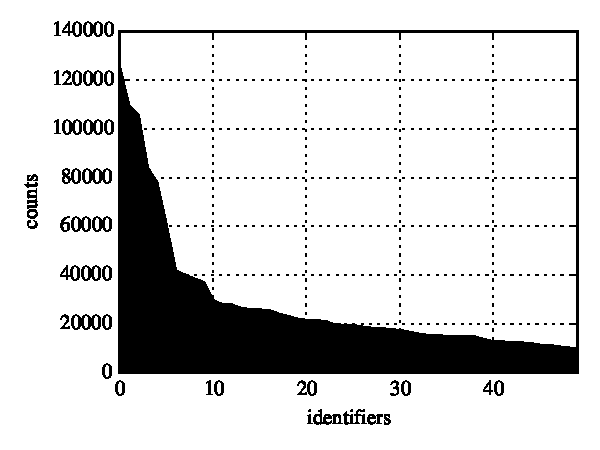
\includegraphics[width=\textwidth]{en-wiki-ids-1.pdf}
  \caption{Frequencies of the first 50 identifiers}
  \label{fig:en-wiki-ids-1}
\end{subfigure}
\hfill
\begin{subfigure}[b]{0.47\textwidth}
  \centering
  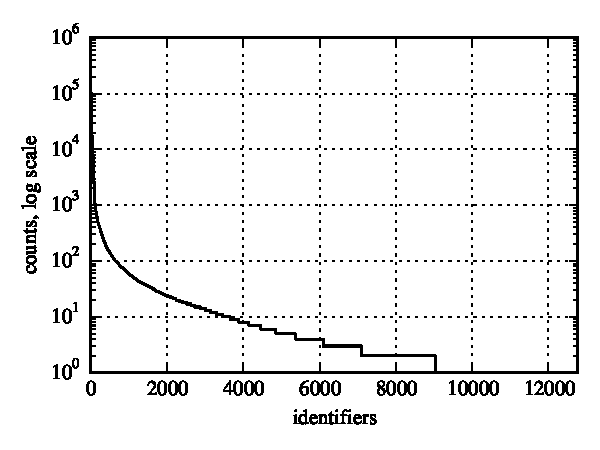
\includegraphics[width=\textwidth]{en-wiki-ids-2-log.pdf}
  \caption{Frequencies, log scale}
  \label{fig:en-wiki-ids-2-log.pdf}
\end{subfigure}
\hfill
\caption{Distribution of frequencies of identifiers}
\label{fig:ed-wiki-ids}
\end{figure}



The distribution of counts for identifiers inside the documents also
appears to follow a long tail power law distribution: there are few articles
that contain many identifiers, while most of the articles do not
(see fig.~\ref{fig:en-wiki-doc-ids-1.pdf}).
The biggest article (``Euclidean algorithm'') has 22\,766 identifiers, a
and the second largest (``Lambda lifting'') has only 6\,500 identifiers.
The mean number of identifiers per document is 33.
The distribution for number of distinct identifiers per document
is less skewed (see fig.~\ref{fig:en-wiki-doc-ids-2.pdf}).
The largest number of distinct identifiers is 287 (in the article
``Hooke's law''), and it is followed by 194 (in ``Dimensionless quantity'').
The median number of identifiers per document is 10.


\begin{figure}[h]
\centering

\begin{subfigure}[b]{\textwidth}
  \centering
  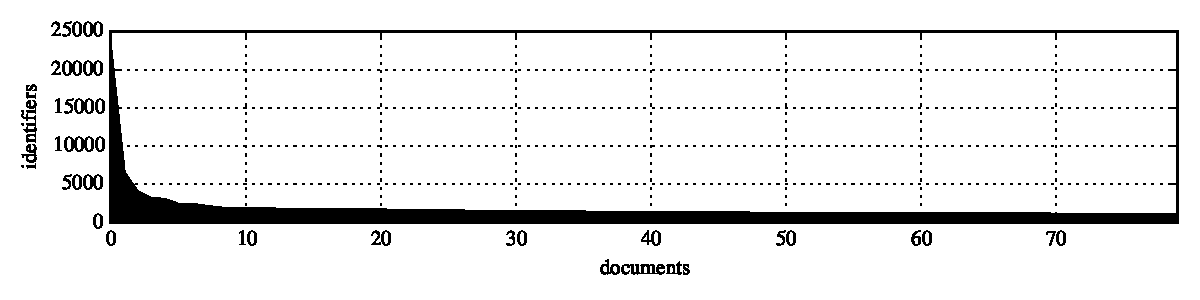
\includegraphics[width=0.9\textwidth]{en-wiki-doc-ids-1.pdf}
  \caption{Identifier frequencies per document for first 80 most largest documents}
  \label{fig:en-wiki-doc-ids-1.pdf}
\end{subfigure}

\begin{subfigure}[b]{\textwidth}
  \centering
  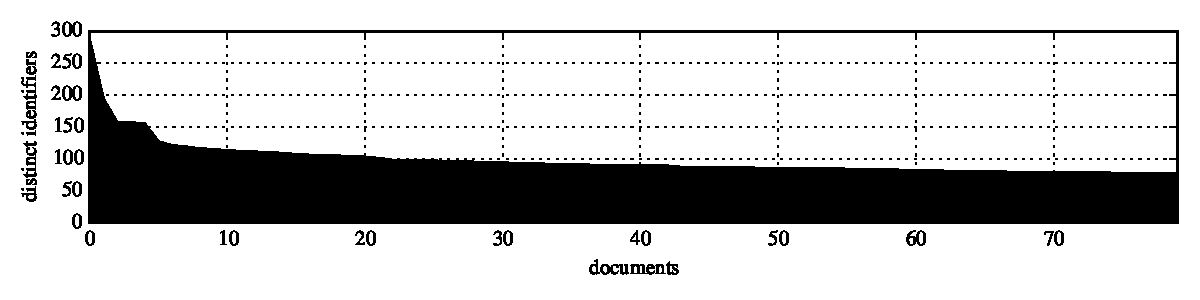
\includegraphics[width=0.9\textwidth]{en-wiki-doc-ids-2.pdf}
  \caption{No. of distinct identifiers per document for first 80 most largest documents}
  \label{fig:en-wiki-doc-ids-2.pdf}
\end{subfigure}

\begin{subfigure}[b]{\textwidth}
  \centering
  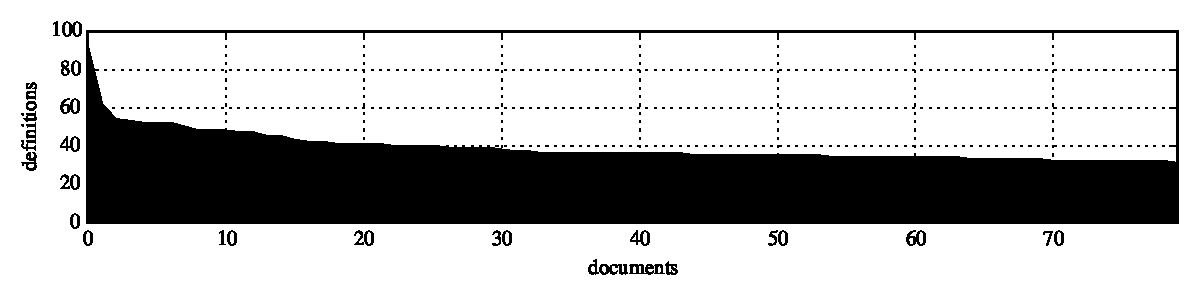
\includegraphics[width=0.9\textwidth]{en-wiki-doc-def.pdf}
  \caption{Definitions per document}
  \label{fig:en-wiki-doc-def.pdf}
\end{subfigure}

\caption{Frequencies per documents}
\label{fig:freqs-doc}

\end{figure}


For 12\,771 identifiers the algorithm extracted 115\,300 definitions, and the
number of found definitions follows a long tail distribution as well
(see fig.~\ref{fig:en-wiki-doc-def.pdf}), with the median number of
definitions per page being 4.

The following is the list of the most common identifier-definition pairs
extracted from English Wikipedia:

\begin{itemize}
\item $t$: ``time'' (1086)
\item $m$: ``mass'' (424)
\item $\theta$: ``angle'' (421)
\item $T$: ``temperature'' (400)
\item $r$: ``radius'' (395)
\item $v$: ``velocity'' (292)
\item $\rho$: ``density'' (290)
\item $G$: ``group'' (287)
\item $V$: ``volume'' (284)
\item $\lambda$: ``wavelength'' (263)
\item $R$: ``radius'' (257)
\item $n$: ``degree'' (233)
\item $r$: ``distance'' (220)
\item $c$: ``speed of light'' (219)
\item $L$: ``length'' (216)
\item $n$: ``length'' (189)
\item $n$: ``order'' (188)
\item $n$: ``dimension'' (185)
\item $n$: ``size'' (178)
\item $M$: ``mass'' (171)
\item $d$: ``distance'' (163)
\item $X$: ``topological space'' (159)
\end{itemize}

In Russian Wikipedia only 5\,300 articles contain enough identifiers,
and the remaining 9\,500 are discarded.

The identifiers and definitions extracted from the Russain version of 
Wikipedia exhibit the similar properties. The most frequently
occurring identifier is $x$ with 13\,248 occurrences,
but the median frequency of an identifer is only 3 times.
The article with the largest number of identifiers is ``��������� ���������''
(``Maxwell's equations'') which contains 1\,831 identifiers, while
the median number of identifiers is just 3;
the article with the largest number of distinct identifiers
is also  ``��������� ���������'' with 112 unique identifiers, and
the median number of distinct identifiers in the data set is 5.
Finally, the largest number of extracted definitions is 44
(again, for ``��������� ���������'') with 2 being the median number of
definitions per page.

The following is the list most frequent relations extracted
from Russian wikipedia:

\begin{itemize}
\item $t$: ``�������'' (``function'') (215)
\item $t$: ``�����'' (``time'') (130)
\item $X$: ``���������'' (``set'') (113)
\item $m$: ``�����'' (``mass'') (103)
\item $c$: ``�������� ����'' (``speed of light'') (89)
\item $G$: ``������'' (``group'') (87)
\item $T$: ``�����������'' (``temperature'') (69)
\item $h$: ``���������� ������'' (``Plank constant'') (68)
\item $\rho$: ``���������'' (``density'') (57)
\item $M$: ``������������'' (``manifold'') (53)
\item $K$: ``����'' (``field'') (53)
\item $X$: ``������������'' (``space'') (50)
\item $v$: ``��������'' (``speed'') (50)
\item $X$: ``�������������� ������������'' (``topological space'') (46)
\item $G$: ``����'' (``graph'') (44)
\item $R$: ``������'' (``radius'') (38)
\item $R$: ``������'' (``ring'') (36)
\item $G$: ``�������������� ����������'' (``gravitational constant'') (34)
\item $E$: ``�������'' (``energy'') (34)
\item $m$: ``������'' (``modulo'') (33)
\item $S$: ``�������'' (``area'') (32)
\item $k$: ``���������� ���������'' (``Boltzmann constant'') (30)
\end{itemize}



\subsection{Document Clustering} \label{sec:clustering-impl}

At the Document Clustering stage we want to find cluster of documents
that are good namespace candidates.

Before we can do this, we need to vectorize our dataset: i.e. build the
Identifier Space (see section~\ref{sec:vsm}) and represent each document
in this space.

There are three choices for dimensions of the Identifier space:

\begin{itemize}
  \item identifiers alone,
  \item ``weak'' identifier-definition association,
  \item ``strong'' association: use identifier-definition pairs.
\end{itemize}

In the first case we are only interested in identifier information and
discard the definitions altogether.

In the second and third cases we keep the definitions and use them to
index the dimensions of the Identifier Space. Bur there is some
variability in the definitions: for example, the same identifier
``$\sigma$'' in one document can be assigned to ``Cauchy stress tensor'' and
in other it can be assigned to ``stress tensor'', which are almost the same thing.
To reduce this variability we perform some preprocessing: we tokenize
the definitions and use individual tokens to index dimensions of the space.
For example, suppose we have two pairs ($\sigma$, ``Cauchy stress tensor'')
and ($\sigma$, ``stress tensor''). In the ``weak'' association case
we have will dimensions $(\sigma, \text{Cauchy}, \text{stress}, \text{tensor})$,
while for the ``strong'' association case we will have
$(\sigma\text{\_Cauchy}, \sigma\text{\_stress}, \sigma\text{\_tensor})$.

Additionally, the effect of variability can be decreased further
by applying a stemming technique for each definition token.
In this work we use Snowball stemmer for English \cite{porter2001snowball}
implemented in NLTK \cite{bird2006nltk}: a python library for
Natural Language Processing. For Russian we use Pymorphy2 \cite{korobov2015morphological}.

Using \verb|TfidfVectorizer|  from  scikit-learn \cite{scikit-learn} we vectorize
each document.

We use the following settings:

\begin{enumerate}[label=\Alph*]
  \item \verb|use_idf=True, min_df=2|
  \item \verb|use_idf=False, min_df=2|
  \item \verb|use_idf=False, sublinear_tf=True, min_df=2|
\end{enumerate}


In the first case we use inverse document frequency (IDF) to assign additional
collection weight for "terms"
(see section~\ref{sec:vsm}), while in second and in third we use only
term frequency (TF).
In the second case we apply a sublinear transformation to the TF component
to reduce  the influence of frequently occurring words.
In all three cases we keep
only "terms" that are used in at least two documents.

The output is a document-identifier matrix (analogous to ``document-term''):
documents are rows and identifiers/definitions are columns.
The output of \verb|TfidfVectorizer| is row-normalized, i.e.
all rows has unit length.


Once we the documents are vectorized, we can apply clustering techniques
to them. We use $K$-Means (see section~\ref{sec:kmeans}) implemented as a 
class \verb|KMeans| in scikit-learn and Mini-Batch $K$-Means (class \verb|MiniBatchKMeans|) \cite{scikit-learn}. Note that if rows are unit-normalized, then running $K$-Means with
Euclidean distance is equivalent to cosine distance
(see section~\ref{sec:cosine}).

Bisecting $K$-Means (see section~\ref{sec:kmeans}) was implemented on top of
scikit-learn: at each step we take a subset of the dataset and apply
$K$-Means with $K = 2$ to this subset. If the subset is big (with number of
documents $n > 2000$), then we use Mini-Batch $K$-means with $K=2$
because it converges much faster.

Scatter/Gather, an extension to $K$-means (see section~\ref{sec:kmeans}), was
implemented manually  using scipy \cite{scipy} and numpy \cite{walt2011numpy} because
scikit-learn's implementation of $K$-Means does not allow using user-defined distances.

DBSCAN (section~\ref{sec:dbscan}) and SNN Clustering (also section~\ref{sec:dbscan})
algorithms were also implemented manually:
available DBSCAN implementations usually take distance measure rather than
a similarity measure. The similarity matrix cleated by similarity measures
are typically very sparse, because usually only a small fraction of the documents
are similar to some given document. Similarity measures
can be converted to distance measures, but in this case
the matrix will no longer be sparse, and we would like to avoid that.
Additionally, available implementations are usually general purpose
implementations and do not take advantage of the structure of the data:
in text-like data clustering algorithms can be sped up significantly
by using an inverted index.


Dimensionality reduction techniques are also important: they
not only reduce the dimensionality, but also help reveal the latent
structure of data. In this work we use Latent Semantic Analysis (LSA) (section~\ref{sec:lsa})
which is implemented using randomized Singular Value Decomposition (SVD)
\cite{tropp2009finding}, The implementation of randomized SVD is taken from scikit-learn
\cite{scikit-learn} -- method \verb|randomized_svd|. Non-negative Matrix Factorization
is an alternative technique for dimensionality reduction (section~\ref{sec:lsa}).
Its implementation is also taken from scikit-learn \cite{scikit-learn},
class \verb|NMF|.

To assess the quality of produced clusters we use wikipedia categories. It is
quite difficult to extract category information from raw wikipedia text,
therefore we use DBPedia \cite{bizer2009dbpedia} for that: it provides
machine-readable information about categories for each wikipedia article.
Additionally, categories in wikipedia form a hierarchy, and this hierarchy
is available as a SKOS ontology.

Unfortunately, there is no information about articles from Russian Wikipedia on 
DBPedia. However the number of documents is not very large, and therefore 
this information can be retrieved via MediaWiki API\footnote{\url{http://ru.wikipedia.org/w/api.php}} individually for each 
document.

\subsubsection{Building Namespaces} \ \\

Once a cluster analysis algorithms assigns documents in our collection to 
some clusters, we need to find namespaces among these clusters. We assume that 
some clusters are namespace-defining: they are not only homogenous in the cluster 
analysis sense (for example, in case of $K$-Means it means that within-cluster sum 
of squares is minimal), but also ``pure'': they are about the same topic. 

A cluster is \emph{pure} if all documents have the same category.
Using categories information we can find the most frequent category of the
cluster, and then we can define purity as
$$\operatorname{purity}(C) = \cfrac{\max_i \operatorname{count}(c_i)}{|C|},$$
where $C$ is a cluster, and $c_i$ is some category. 
Thus we can select all clusters with purity above some pre-defined threshold 
and refer to them as namespace-defining clusters. 

Then we convert these clusters into namespaces by collecting all the identifiers 
and their definitions in the documents of each cluster. To do this, we first 
collect all the identifier-definition pairs, and then group them by identifier. 
When extracting, each definition candidate is scored, and this score is used 
to determine, which definition an identifier will be assigned in the namespace. 

For example, consider three documents with the following extracted relations:

\begin{itemize}
  \item Document A:
  \begin{itemize}
\item $n$: (predictions, 0.95), (size, 0.92), (random sample, 0.82), (population, 0.82)
\item $\theta$: (estimator, 0.98), (unknown parameter, 0.98), (unknown parameter, 0.94)
\item $\mu$: (true mean, 0.96), (population, 0.89)
\item $\mu_4$: (central moment, 0.83)
\item $\sigma$: (population variance, 0.86), (square error, 0.83), (estimators, 0.82)
  \end{itemize}

  \item Document B:
    \begin{itemize}
\item $P_\theta$: (family, 0.87)
\item $X$: (measurable space, 0.95)
\item $\theta$: (sufficient statistic, 0.93)
\item $\mu$: (mean, 0.99), (variance, 0.95), (random variables, 0.89), (normal, 0.83)
\item $\sigma$: (variance, 0.99), (mean, 0.83)
  \end{itemize}

  \item Document C:
    \begin{itemize}
\item $n$: (tickets, 0.96), (maximum-likelihood estimator, 0.89)
\item $x$: (data, 0.99), (observations, 0.93)
\item $\theta$: (statistic, 0.95), (estimator, 0.93), (estimator, 0.93), (rise, 0.91), (statistical model, 0.85), (fixed constant, 0.82)
\item $\mu$: (expectation, 0.96), (variance, 0.93), (population, 0.89)
\item $\sigma$: (variance, 0.94), (population variance, 0.91), (estimator, 0.87)
  \end{itemize}
\end{itemize}

We take all these relations, and combine together. If an identifer 
have two or more definitions that are exactly the same, them we 
merge them into one and its score is the sum of scores: 

\begin{itemize}
\item $P_\theta$: (family, 0.87)
\item $X$: (measurable space, 0.95), (Poisson, 0.82)
\item $n$: (tickets, 0.96), (predictions, 0.95), (size, 0.92), (maximum-likelihood estimator, 0.89), (random sample, 0.82), (population, 0.82)
\item $x$: (data, 0.99), (observations, 0.93)
\item $\theta$: (estimator, 0.98+0.93+0.93), (unknown parameter, 0.98+0.94), (statistic, 0.95), (sufficient statistic, 0.93), (rise, 0.91), (statistical model, 0.85), (fixed constant, 0.82)
\item $\mu$: (random variables, 0.89+0.89+0.89), (variance, 0.95+0.93), (mean, 0.99), (true mean, 0.96), (expectation, 0.96), (normal, 0.83)
\item $\mu_4$: (central moment, 0.83)
\item $\sigma$: (variance, 0.99+0.94), (population variance, 0.91+0.86), (estimator, 0.87), (square error, 0.83), (mean, 0.83), (estimators, 0.82)
\end{itemize}

There is some lexical variance in the definitions. For example, ``variance'' and ``population
variance'' or ``mean'' and ``true mean'' are very related definitions, and 
it makes sense to group them together to form one definition. 
It can be done by fuzzy string matching (or approximate matching)
\cite{navarro2001guided}. To implement it, we use a python library FuzzyWuzzy 
\cite{fuzzywuzzy}, and using fuzzy matching we group related identifiers and then 
sum over their scores. 

Then we have the following: 

\begin{itemize}
\item $P_\theta$: (family, 0.87)
\item $X$: (measurable space, 0.95), (Poisson, 0.82)
\item $n$: (tickets, 0.96), (predictions, 0.95), (size, 0.92), (maximum-likelihood estimator, 0.89), (random sample, 0.82), (population, 0.82)
\item $x$: (data, 0.99), (observations, 0.93)
\item $\theta$: (estimator, 2.84), (unknown parameter, 1.92), (\{statistic, sufficient statistic\}, 1.88), (rise, 0.91), (statistical model, 0.85), (fixed constant, 0.82)
\item $\mu$: (random variables, 2.67), (\{mean, true mean\}, 1.95), (variance, 1.88),  (expectation, 0.96), (normal, 0.83)
\item $\mu_4$: (central moment, 0.83)
\item $\sigma$: (\{variance, population variance\}, 3.7), (\{estimator, estimators\}, 1.69), (square error, 0.83), (mean, 0.83)
\end{itemize}

In a namespace an identifier can have at most one definition, and therefore the next step 
is selecting the definition with the highest score. This gives us the following namespace: 

\begin{itemize}
\item ($P_\theta$, family, 0.87)
\item ($X$, measurable space, 0.95)
\item ($n$, tickets, 0.96)
\item ($x$, data, 0.99
\item ($\theta$, estimator, 2.84)
\item ($\mu$, random variables, 2.67)
\item ($\mu_4$, central moment, 0.83)
\item ($\sigma$: variance, 3.7)
\end{itemize}


The category of this namespace is selected as the category that the majority of the documents 
in the namespace-defining cluster share.


\subsection{Experiments} \label{sec:param-tuning} 

There are many different clustering algorithms, each with its own set
of parameter. In this section we describe how we find the settings that
find the best namespaces.

The following things can be changed:

\begin{itemize}
  \item Ways to incorporate definition information (no definitions, soft association, hard association);
  \item Weighting schemes for the identifier-document matrix $D$: TF, sublinear TF, TF-IDF;
  \item There are different clustering algorithms: agglomerative clustering, DBSCAN, SNN clustering, $K$-Means, Bisecting $K$-Means, each algorithm has its own set of parameters;
  \item Dimensionality of $D$ can be reduced via SVD or NMF, parameter $k$ controls the rank of output.
\end{itemize}

% The approach for finding
% Distance and similarity measures used
% Euclidean distance, cosine similarity, jaccard similarity, SNN Similarity

To find the best parameters set we use the grid search approach: we try
different combinations of parameters and keep track on the number of
pure clusters and the purity.

The overall 
purity of cluster assignment is calculated as a weighed sum of individual 
cluster purities, where the weight is chosen proportionally to the size of a
cluster.

However it is not
enough just to find the most pure cluster assignment: because as the number
of clusters increases the overall purity also grows.
Thus we can also optimize for the number of clusters with purity $p$ of
size at least $n$.

When the number of clusters increase, the purity always grows
(see fig.~\ref{fig:k-vs-purity}), but at some point the number of pure clusters
will start decreasing (see fig.~\ref{fig:k-vs-pureclusters}).

\begin{figure}[h!]
\centering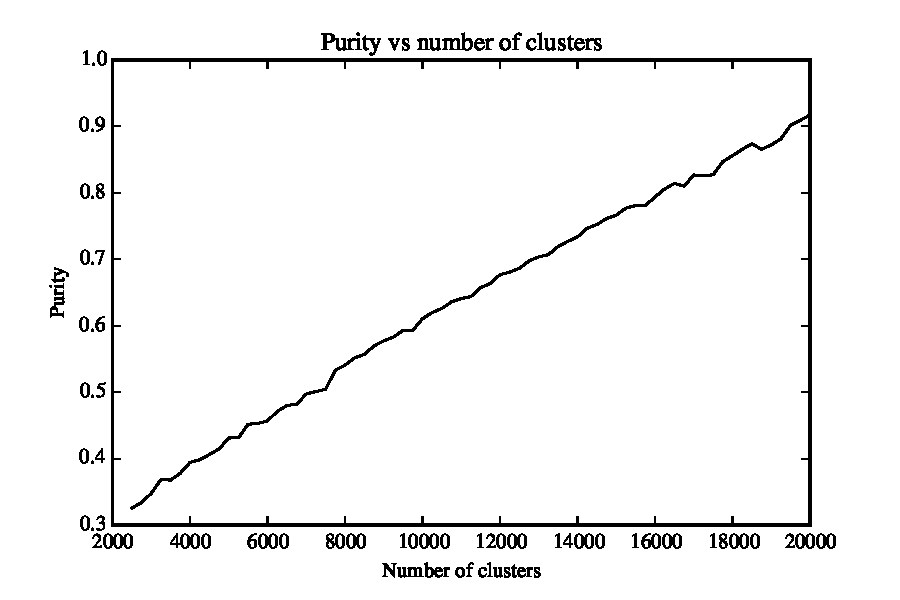
\includegraphics[width=0.8\textwidth]{purity.pdf}
\caption{$K$ in $K$-Means vs overall purity of clustering: the purity increases
linearly with $K$ ($R^2 = 0.99$).}
\label{fig:k-vs-purity}
\end{figure}

\begin{figure}[h!]
\centering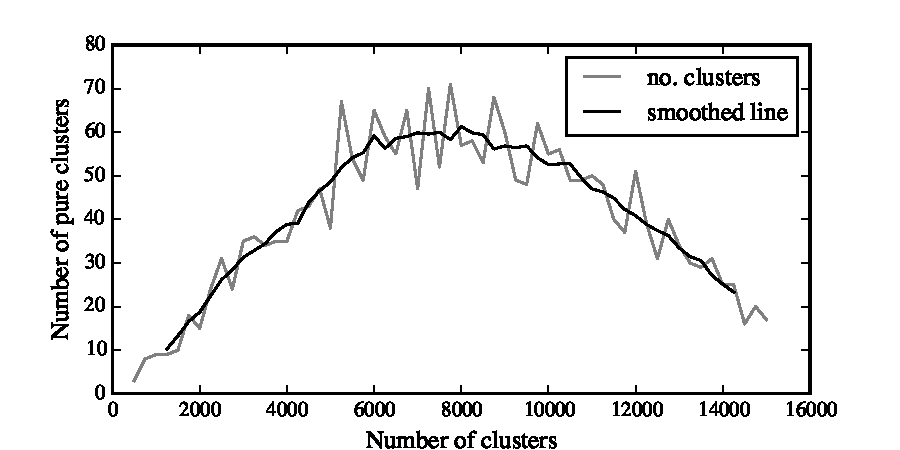
\includegraphics[width=0.8\textwidth]{pure-clusters.pdf}
\caption{$K$ in $K$-Means vs the number of pure clusters: it grows initially, but after $K\approx 8\,000$ starts to decrease.}
\label{fig:k-vs-pureclusters}
\end{figure}


\subsubsection{Baseline} \ \\

We compare the performance of clustering algorithms against a random
categorizer. The simplest version of such a categorizer is the random 
cluster assignment categorizer, which assigns each document to some random
cluster. 
In this case, we constrain the categorizer to include 3 documents in each 
cluster, and once a document belongs to some cluster, it cannot be re-assigned. 
It is done by first creating a vector of assignments and shuffling it.

Then we record how many pure clusters (at least 80\% pure) are in the cluster
assignment.

We repeated this experiment for 200 times (see fig.~\ref{fig:baseline}): the maximal 
achieved value is 39, while the mean value is 23.85.

\begin{figure}[h!]
\centering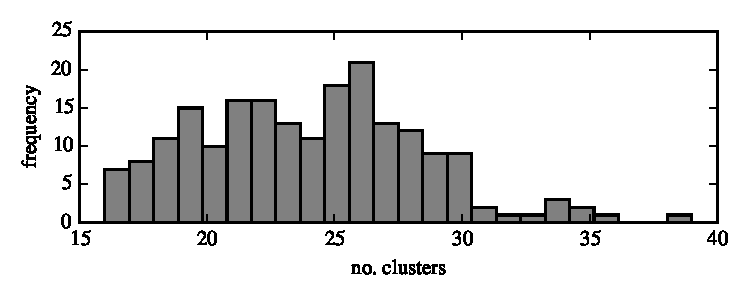
\includegraphics[width=0.7\textwidth]{baseline.pdf}
\caption{Distribution of the number of pure clusters across 200 trials.}
\label{fig:baseline}
\end{figure}


% \textbf{TODO }Also: experiment with not just three, but with some 
% probability distribution say clusters can vary from 3 to 10 or whatever.



\subsubsection{Only Identifiers} \ \\

The first way of building the identifier space is to use only identifiers
and do not use definitions at all.

If we do this, the identifier-document matrix is $6075 \times 22512$ 
(we keep only identifiers that occur at least twice), and it contains  302\, 541
records, so the density of this matrix is just 0.002.

First, we try to apply agglomerative clustering, then DBSCAN with SNN similarity 
based on Jaccard coefficient and cosine similarity, then we 
do $K$-Means and finally we apply LSA using SVD and NMF and apply 
$K$-Means on the reduced space. 

\textbf{Agglomerative clustering} take too long to compute, they were not able 
to finish clustering in several hours, so we stopped the computation 
(\textbf{add graphs}). Additionally, the implementation we use from scikit-learn 
require a dense matrix, when densified, the identifeir-document matrix 
occupies a lot of space. Therefore we exclude these clustering algorithms from
further analysis.
% Agglomerative: Wald linkage: takes forever never finished


The second method is \textbf{DBSCAN} with \textbf{SNN Similarity}. 
To compute SSN similarity we need to use some other base similarity measure. 
We start with Jaccard coefficient, and use a binarized identifier-document 
matrix: a matrix with only ones and zeros.  
For example, the closest article to ``Linear Regression'' is 
``Linear predictor function'' with Jaccard coefficient of 0.59
and ``Low-rank approximation'' is the closest to ``Singular value decomposition''
with coefficient of 0.25. With Jaccard, we were able to discover 87 
clusters, which is two times better than the baseline (see fig.~\ref{fig:nodef-dbscan-jac})
and the best parameters are 10 nearest neighbors, 
$\varepsilon=3$ and \texttt{MinPts} $=4$ (see fig.~\ref{fig:nodef-dbscan-jac10-2}).

For the best result with 87 namespace defining clusters, 
in total 5\,580 clusters were found and 4\,219 documents are considered
as ``noise''. Let us consider top largest found clusters (see table~\ref{tab:nodef-jaccard}). 
One of them, ``Statistics'',  is quite homogenous with purity of 0.84 (see table~\ref{tab:nodef-jaccard-stat}).
Although some of the articles in this cluster are not related to statistics, 
all of them articles share the same identifier ``$\beta$''. 
We can also check how $\beta$ is defined across all namespace-defining clusters 
(see table~\ref{tab:nodef-jaccard-beta}). There are not many instance of 
$\beta$, and not all of them correct or meaningful: for example  ``i/ab'' in 
the ``Physics'' cluster is a non-definition that was not successfully filtered 
out during the data cleaning phase.

\begin{table}[h!]
\centering
\begin{tabular}{|c|c|c|}
  \hline
  Name & Size & Purity \\
  \hline
Continuum mechanics & 40 & 0.8000 \\
Constellations listed by Ptolemy & 17 & 1.0000 \\
Statistics & 13 & 0.8462 \\
Knot theory & 13 & 0.8462 \\
Electromagnetism & 12 & 0.8333 \\
Bayer objects & 11 & 1.0000 \\
Analytic number theory & 10 & 0.9000 \\
Acoustics & 9 & 0.8889 \\
Chemical properties & 9 & 0.8889 \\
Set theory & 9 & 0.8889 \\
Combinatorics & 8 & 0.8750 \\
Theory of computation & 8 & 1.0000 \\
Partial differential equations & 8 & 0.8750 \\
Mathematical logic & 8 & 0.8750 \\
\hline
\end{tabular}
\caption{Top namespace-defining clusters discovered by SNN DBSCAN with Jaccard coefficient.}
\label{tab:nodef-jaccard}
\end{table}

\begin{table}[h!]
\centering
\begin{subtable}{0.65\textwidth}
\centering
\begin{tabular}{|c|c|}
\hline
Article Name & Identifiers \\
\hline
Partition of sums of squares & $y, \beta_0, \beta_1, \varepsilon_i, \beta_p, S, \varepsilon, y_i, \beta, ...$ \\
Deming regression & $\sigma, \eta, \eta_i, \beta, \beta_0, \varepsilon_i, \varepsilon, \delta, y_i, x, ...$ \\
Instrumental variable & $\beta, \varepsilon, \delta, x_1, Y, X,g, f, \varepsilon_i, \beta_k, ...$ \\
Ordinary least squares &w_i, \alpha, \beta, \varepsilon, \sigma, E, \eta, \chi, \varepsilon_i,  \beta_j, ...$ \\
Endogeneity & $\gamma, \varepsilon_i, \beta_1, x_i, \alpha, \beta, \varepsilon, ...$ \\
Linear predictor function & $x_i, \varepsilon_2, \beta_0,  \varepsilon_1, \beta, \varepsilon, \phi_p, \varepsilon_n, ...$ \\
Stochastic frontier analysis & $\beta_n, f, \beta_0, u_i, x_i, \beta, T, y_i, ...$ \\
\begin{tabular}[x]{@{}c@{}} Proofs involving \\ ordinary least squares \end{tabular} &
  $x_i, \beta_0, \beta_1, \beta, \varepsilon, \pi, \sigma, \chi, \varepsilon_i, ...$ \\
Projection pursuit regression & $\beta, \beta_0, j, S, \varepsilon, y_i, X, Y, x, x_i, ...$ \\
De Casteljau's algorithm & $w_i, \beta_0, \beta_1,  \beta, \beta_i, t, \beta_n, t_0, P_0, ...$ \\
Regression analysis & $x_i, \beta_0, \beta, \varepsilon, y_i, \sigma, f, \beta_p, \varepsilon_i, ...$ \\
Linear regression & $x_i, \varepsilon_2, \Omega, \beta_1, \beta_2, y_n, \varepsilon_1, \beta, \varepsilon, ...$ \\
Least squares & $\nabla, \beta_j, \beta, \varepsilon, w_{ii}, Wy, \sigma, \varepsilon_i, ...$ \\
\hline
\end{tabular}
\label{tab:nodef-jaccard-docs}
\caption{Identifiers and articles of the ``Statistics'' cluster (some identifiers are removed)}
\end{subtable}% mask EOL
\begin{subtable}{0.3\textwidth}
\centering
\begin{tabular}{|c|c|c|}
\hline
ID & Definition & Score\\
\hline
$X_1$ & regressors & 0.92 \\
$Y$ & regression model & 0.95 \\
$f$ & linear predictor function & 0.99 \\
$p$ & regressors & 1.77 \\
$w_i$ & control points & 1.66 \\
$y_0$ & mean response & 0.99 \\
$y_i$ & dependent variable & 3.71 \\
$z$ & causal relationship & 0.90 \\
$\alpha$ & confidence level & 1.94 \\
$\beta$ & estimator & 2.82 \\
$\beta_1$ & slope & 1.82 \\
$\varepsilon$ & errors & 2.90 \\
$\varepsilon_i$ & error term & 2.71 \\
$\sigma$ & residual variance & 2.68 \\
\hline
\end{tabular}
\label{tab:nodef-jaccard-ids}
\caption{Definitions in ``Statistics'' (some definitions are removed)}
\end{subtable}
\caption{A namespace-defining cluster about Statistics dicovered by SNN DBSCAN 
with Jaccard coefficient.}
\label{tab:nodef-jaccard-stat}
\end{table}



\begin{table}[h!]
\centering
\begin{tabular}{|c|c|c|c|}
  \hline
  \multicolumn{4}{|c|}{$\beta$}\\
  \hline
  Size & Namespace Name & Definition & Score \\
  \hline
3 & Complex analysis & absolute value & 0.95 \\
40 & Continuum mechanics & bias & 1.75 \\
5 & Fluid dynamics & momentum factor & 0.95 \\
5 & Physics & i/ab & 0.84 \\
3 & Quantum mechanics & voltage-to-barrier-field conversion factor & 1.87 \\
5 & Radio frequency propagation & clutter factor & 0.95 \\
9 & Set theory & successor ordinal & 0.89 \\
13 & Statistics & estimator & 2.82 \\
6 & Theoretical physics & quantity & 0.96 \\
\hline
\end{tabular}
\caption{Definitions of $\beta$ in the namespaces discovered by SNN DBSCAN with Jaccard coefficient.}
\label{tab:nodef-jaccard-beta}
\end{table}


\begin{figure}[h!]
\centering
\begin{subfigure}[b]{0.5\textwidth}
  \centering
  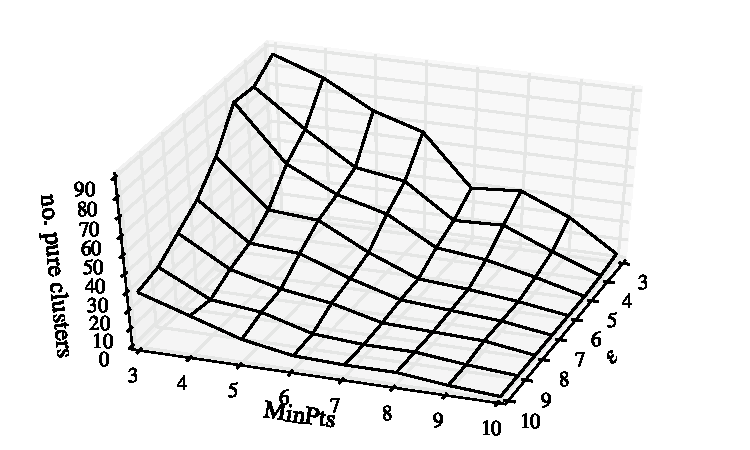
\includegraphics[width=\textwidth]{nodef-dbscan-jac10.pdf}
  \caption{Number of clusters when 10 nearest neighbors are considered}
  \label{fig:nodef-dbscan-jac10}
\end{subfigure}%
\begin{subfigure}[b]{0.5\textwidth}
  \centering
  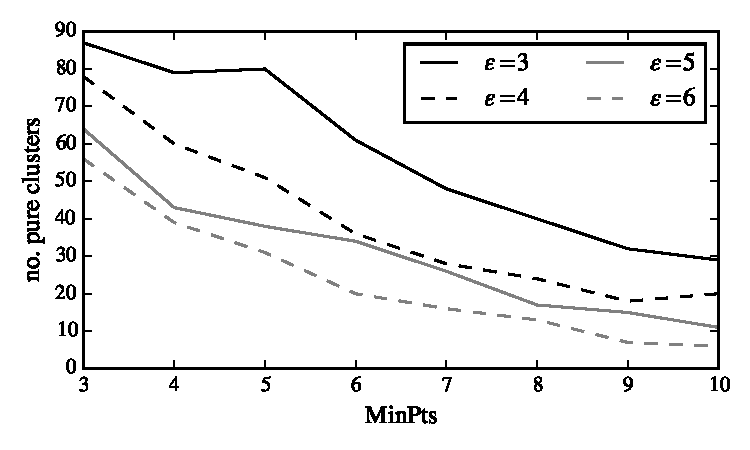
\includegraphics[width=\textwidth]{nodef-dbscan-jac10-2.pdf}
  \caption{Performance of selected $\varepsilon$ with 10 nearest neighbors}
  \label{fig:nodef-dbscan-jac10-2}
\end{subfigure}
\begin{subfigure}[b]{0.5\textwidth}
  \centering
  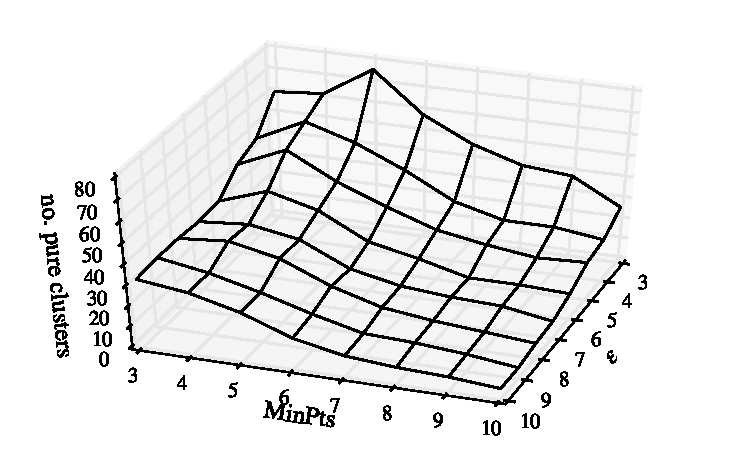
\includegraphics[width=\textwidth]{nodef-dbscan-jac13.pdf}
  \caption{Number of clusters when 15 nearest neighbors are considered}
  \label{fig:nodef-dbscan-jac15}
\end{subfigure}%
\begin{subfigure}[b]{0.5\textwidth}
  \centering
  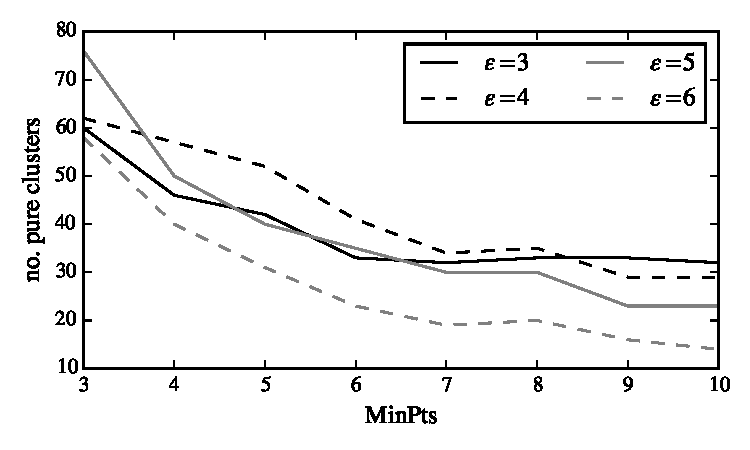
\includegraphics[width=\textwidth]{nodef-dbscan-jac13-2.pdf}
  \caption{Performance of selected $\varepsilon$ with 15 nearest neighbors}
  \label{fig:nodef-dbscan-jac15-2}
\end{subfigure}
\caption{Effect of parameters $\varepsilon$, \texttt{MinPts} and number of nearest
 neighbors on performance of SNN DBSCAN when Jaccard coefficient is used.}
\label{fig:nodef-dbscan-jac}
\end{figure}


Then we run the same algorithm, but with cosine similarity, using an 
identifier-document matrix with $\log \text{TF} \times \text{IDF}$ 
weights, and calculate pair-wise similarity between each document. 
For example, let us take an article ``Linear regression''
%it contains $h_i, m, n, p, T, t, t_i, X, x, x_{11},$ $x_{21}, x_i, y, y_1,$ 
%$y_2, y_i, y_n, Z,  \beta, \beta_1, \beta_2, \beta_p, \varepsilon, \varepsilon_1, 
%\varepsilon_2,$ $\varepsilon_i, \varepsilon_n, \Omega$
and calculate the cosine with the rest of the corpus. The closest document 
is ``Linear predictor function''.
% with identifiers
%$b, c, c_1, f, m, p1, T, x, X,$ $x_{11}, x_i, x_K, y, y_2, y_i, y_n, \beta_0, 
%\beta_1, \beta_2, \beta_p, \beta 2, \varepsilon,$ $\varepsilon_1, \varepsilon_2, \varepsilon_i,$
%$\phi, \phi_1, \phi_2$.
They have 23 identifiers in common, and they indeed look related. 
However cosine is not always giving the best closets neighbors. For example,
the nearest neighbor of ``Singular value decomposition'' is ``Rule of Sarrus'', 
and although their cosine score is 0.92, they have only 3 identifiers in common.  

\begin{figure}[h!]
\centering
\begin{subfigure}[b]{0.5\textwidth}
  \centering
  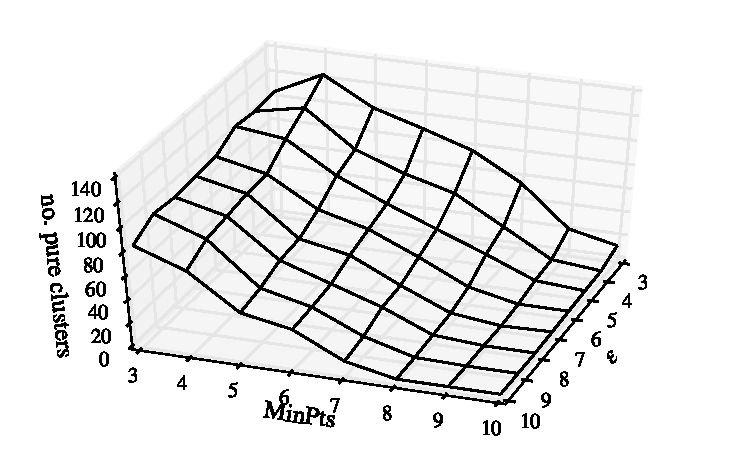
\includegraphics[width=\textwidth]{nodef-dbscan-cos10.pdf}
  \caption{Number of clusters when 10 nearest neighbors are considered}
  \label{fig:nodef-dbscan-cos10}
\end{subfigure}%
\begin{subfigure}[b]{0.5\textwidth}
  \centering
  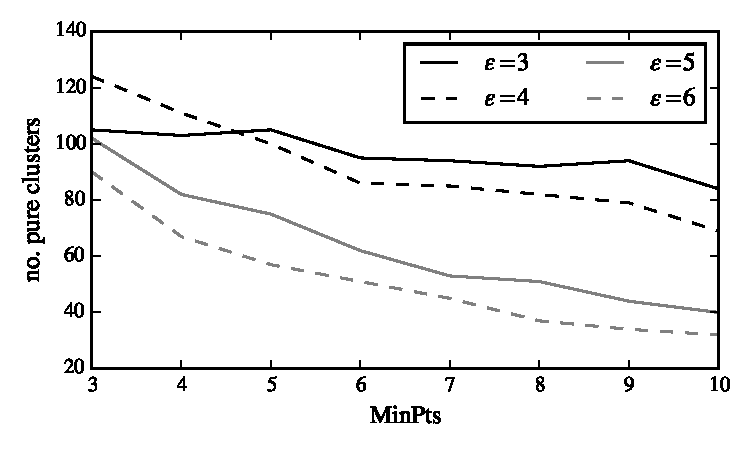
\includegraphics[width=\textwidth]{nodef-dbscan-cos10-2.pdf}
  \caption{Performance of selected $\varepsilon$ with 10 nearest neighbors}
  \label{fig:nodef-dbscan-cos10-2}
\end{subfigure}
\begin{subfigure}[b]{0.5\textwidth}
  \centering
  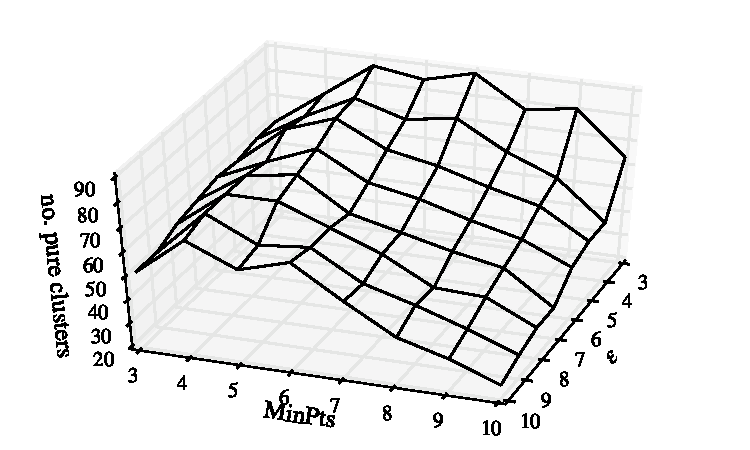
\includegraphics[width=\textwidth]{nodef-dbscan-cos15.pdf}
  \caption{Number of clusters when 15 nearest neighbors are considered}
  \label{fig:nodef-dbscan-cos15}
\end{subfigure}%
\begin{subfigure}[b]{0.5\textwidth}
  \centering
  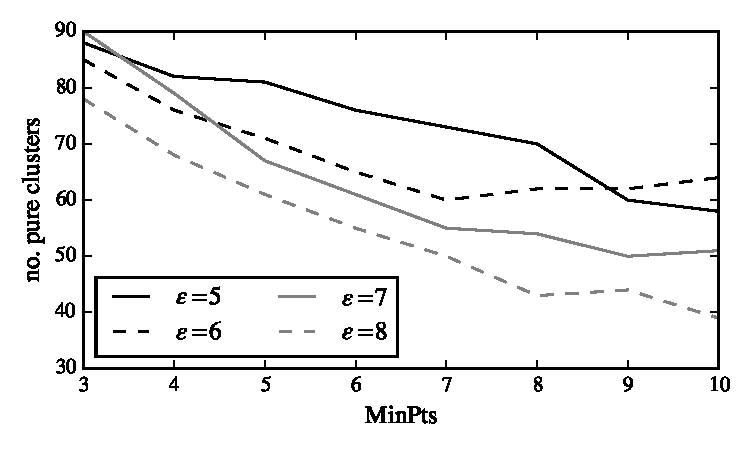
\includegraphics[width=\textwidth]{nodef-dbscan-cos15-2.pdf}
  \caption{Performance of selected $\varepsilon$ with 15 nearest neighbors}
  \label{fig:nodef-dbscan-cos15-2}
\end{subfigure}
\caption{Effect of parameters $\varepsilon$, \texttt{MinPts} and number of nearest
 neighbors on performance of SNN DBSCAN when cosine is used.}
\label{fig:nodef-dbscan-cos}
\end{figure}


With cosine as the base similarity function for SNN DBSCAN we 
were able to discover 124 namespace-defining clusters (see fig.~\ref{fig:nodef-dbscan-cos}),
which is significantly better than the baseline. The best parameters 
are 10 nearest neighbors and $\varepsilon=4$, \texttt{MinPts} $=3$
(see fig.~\ref{fig:nodef-dbscan-cos10-2}).


\begin{figure}[h!]
\centering
\begin{subfigure}[b]{0.75\textwidth}
  \centering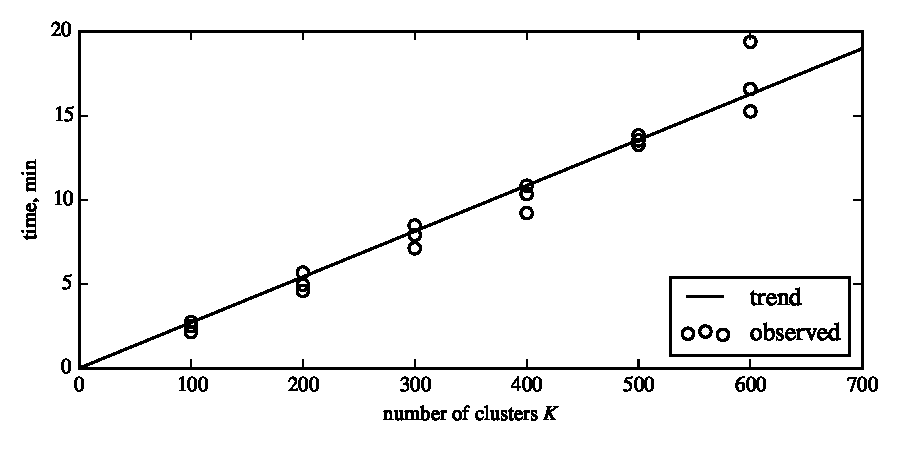
\includegraphics[width=\textwidth]{k-vs-time.pdf}
  \caption{$K$ in $K$-Means vs time in minutes ($R^2 = 0.99$).}
  \label{fig:k-vs-time}
\end{subfigure}

\begin{subfigure}[b]{0.75\textwidth}
  \centering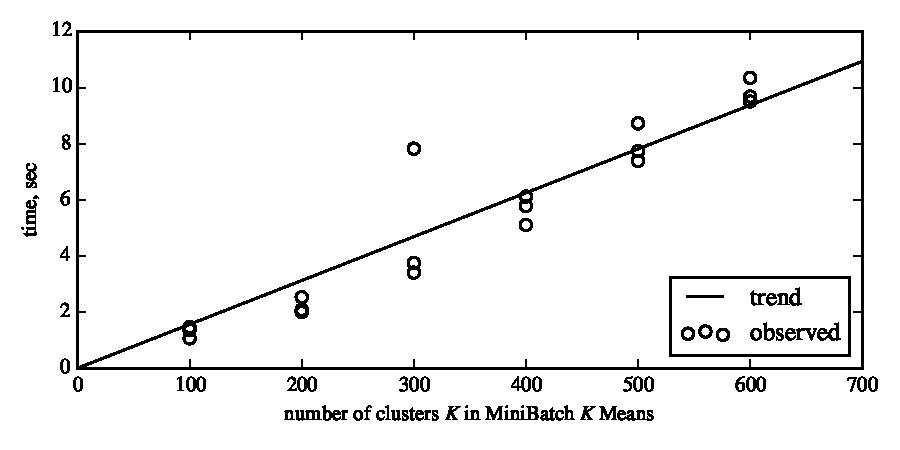
\includegraphics[width=\textwidth]{k-vs-time-minibatch.pdf}
  \caption{$K$ in MiniBatch $K$-Means vs time in seconds ($R^2 = 0.97$).}
  \label{fig:k-vs-time-minibatch}
\end{subfigure}
\caption{Runtime of $K$-Means and MiniBatch $K$-Means}
\label{fig:kmeans-vs-minibatch1}
\end{figure}

Next, we apply \textbf{$K$-Means}. We observe that increasing~$K$ 
leads to linear increase in time (see fig.~\ref{fig:k-vs-time}),
which means that for bigger values of~$K$, it takes longer, so it is not
feasible to run: for example, $K = 10\, 000$ we estimate the runtime to be
about 4.5 hours. As \textbf{MiniBatch $K$-Means} is expected to be significantly 
faster than usual $K$-Means, we use it as well. Although we observe that the run 
time of  MiniBatch $K$-Means also increases linearly with~$K$
(see fig.~\ref{fig:k-vs-time-minibatch}), it indeed runs considerably faster.
For example, MiniBatch $K$-Means takes 15 seconds with $K=700$ while
usual $K$-Means takes about 15 minutes (see fig.~\ref{fig:k-vs-time}
and fig.~\ref{fig:k-vs-time-minibatch}).



Usual $K$-Means with small $K$ does not find many good and pure clusters,
and MiniBatch $K$-Means does even worse: no matter what $K$ is selected,
the number of pure clusters and purity does not change much (see fig.~\ref{fig:k-vs-purity2}
and fig.~\ref{fig:k-vs-len2}). This is also true for larger values of $K$
(see fig.~\ref{fig:k-vs-len-mb}).


% to the end of subsubsection?
%We can conclude that although MiniBatch $K$-Means is
%very fast, it does not perform well on the untransformed data when we don't use
%definitions.



\begin{figure}[h!]
\centering
\hfill
\begin{subfigure}[b]{0.5\textwidth}
  \centering
  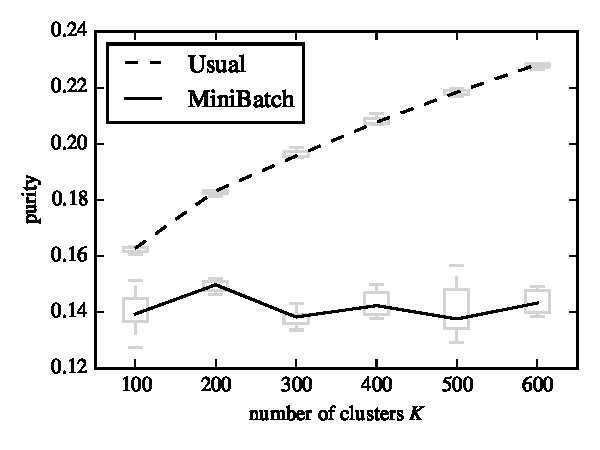
\includegraphics[width=\textwidth]{k-vs-purity2.pdf}
  \caption{Purity vs number of clusters $K$ in \mbox{$K$-Means} and MiniBatch $K$-Means}
  \label{fig:k-vs-purity2}
\end{subfigure}%
\begin{subfigure}[b]{0.5\textwidth}
  \centering
  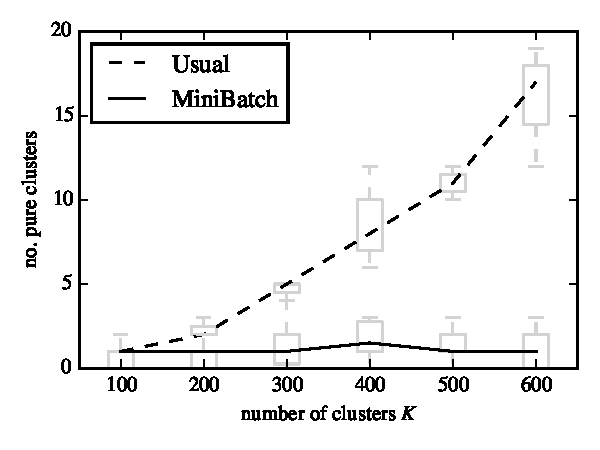
\includegraphics[width=\textwidth]{k-vs-len2.pdf}
  \caption{Number of pure clusters vs $K$ in $K$-Means and MiniBatch $K$-Means}
  \label{fig:k-vs-len2}
\end{subfigure}
\hfill
\begin{subfigure}[b]{\textwidth}
  \centering
  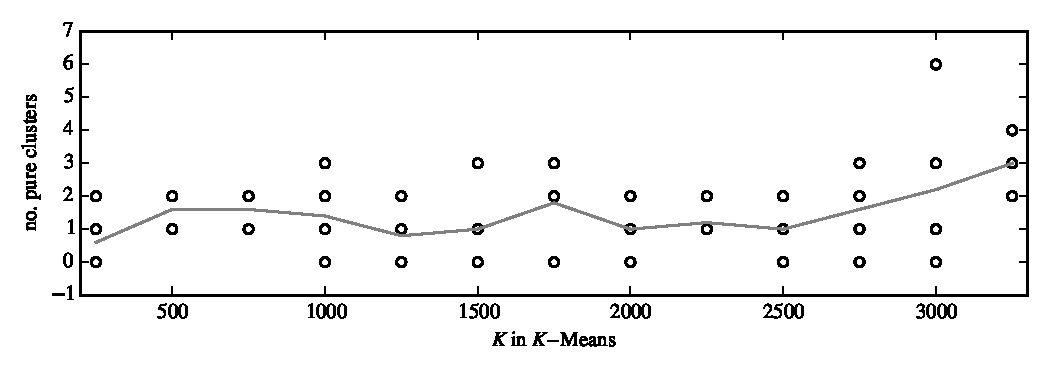
\includegraphics[width=0.85\textwidth]{k-vs-len-mb.pdf}
  \caption{Number of pure clusters vs $K$ in MiniBatch $K$-Means for larger $K$}
  \label{fig:k-vs-len-mb}
\end{subfigure}
\hfill
\caption{Effect of $K$ on performance in $K$-Means}
\label{fig:kmeans-vs-minibatch}
\end{figure}


The best result was found by usual $K$-Means with $K=600$: it was able
to discover 19 clusters with purity at least 0.8 (note that this is worse 
than the baseline of 39 pure clusters). Although it is not many,
the found clusters are very tight and quite big.
Among others, it discovered the following clusters: ``Astronomical catalogues'' (53 documents)
``Stochastic processes'' (39 documents), ``Theory of computation'' (17 documents),
``Thermodynamics'' (16 documents), ``Statistics'' (13 documents).
For example, the cluster ``Astronomical catalogues'' (see table~\ref{tab:kmeans-stars})
primarily constants documents about stars, and all these documents share
the same set of identifers $(p, R_*, m, R_\odot)$.

\begin{table}[h!]
\centering
\begin{tabular}{|c|c|}
\hline
Article & Identifiers \\
\hline
Beta Columbae & $p, R_*, m, R_\odot$ \\
Eta Pegasi & $p, R_*, m, R_\odot$ \\
Sigma Puppis & $p, R_*, m, R_\odot$ \\
Gamma Ceti & $p, R_*, m, R_\odot$ \\
Epsilon Corvi & $p, R_*, m, R_\odot$ \\
Beta Corvi & $p, R_*, m, R_\odot$ \\
Gamma Herculis & $p, R_*, m, R_\odot$ \\
Psi2 Aurigae & $p, R_*, m, R_\odot$ \\
Psi7 Aurigae & $p, R_*, m, R_\odot$ \\
Epsilon Sagittarii & $p, R_*, m, R_\odot$ \\
Alpha Gruis & $p, R_*, m, R_\odot$ \\
Theta Centauri & $p, R_*, m, R_\odot$ \\
... & ... \\
\hline
\end{tabular}
\caption{Stars cluster discovered by $K$-Means}
\label{tab:kmeans-stars}
\end{table}

Next, we use \textbf{Latent Semantic Analysis} with \textbf{SVD}
to reduce the dimensionality of the identifier-document
matrix $D$, and then apply $K$-Means on the reduced space. As discussed in the 
LSA section (see section~ref), it should reveal the latent structure of data. 
We expect that it should improve the results achieved by usual $K$-Means.

Randomized SVD is very fast, but the runtime does not grow linearly with $k$,
it looks quadratic (see fig.~\ref{fig:k-svd-vs-time}).
However, the typical values of $k$ for SVD used in latent semantic analysis is
150-250 \cite{aggarwal2012survey} \cite{evangelopoulos2012latent},
therefore the run time is not prohibitive, and we do not need to rut it
with very large $k$.

\begin{figure}[h!]
\centering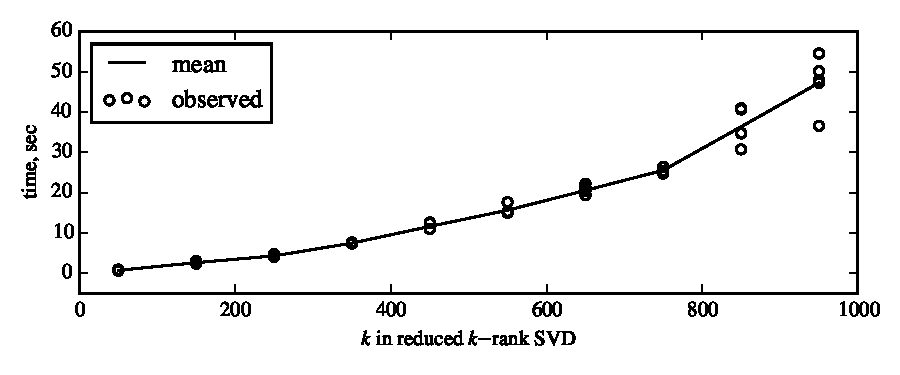
\includegraphics[width=0.75\textwidth]{k-svd-vs-time.pdf}
\caption{$k$ in $k$-rank-reduced randomized SVD vs time in seconds.}
\label{fig:k-svd-vs-time}
\end{figure}


When the dimensionality is reduced, the performance of $K$-Means and
MiniBatch $K$-Means is similar (see fig.~\ref{fig:k-vs-mb-svd-purity}),
but with MiniBatch $K$-Means we were able to discover more interesting pure
clusters (see fig.~\ref{fig:k-vs-mb-svd-len}). The reason for this may be the fact that in the reduced space there is less noise and both methods find equally good clusters,
but because MiniBatch $K$-Means works faster, we are able to run it multiple
times thus increasing its chances to find a good local optimum where there
are many pure document clusters. Note that the obtained result is below 
the baseline.


\begin{figure}[h!]
\centering
\hfill
\begin{subfigure}[b]{0.47\textwidth}
  \centering
  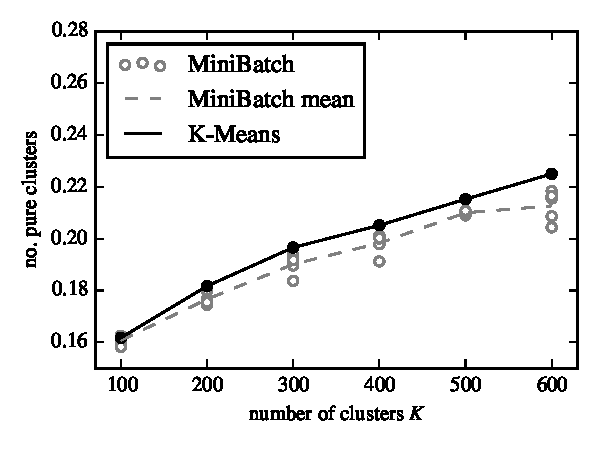
\includegraphics[width=\textwidth]{k-vs-mb-svd-purity.pdf}
  \caption{Purity vs number of clusters $K$ in \mbox{$K$-Means} and MiniBatch $K$-Means}
  \label{fig:k-vs-mb-svd-purity}
\end{subfigure}
~
\begin{subfigure}[b]{0.47\textwidth}
  \centering
  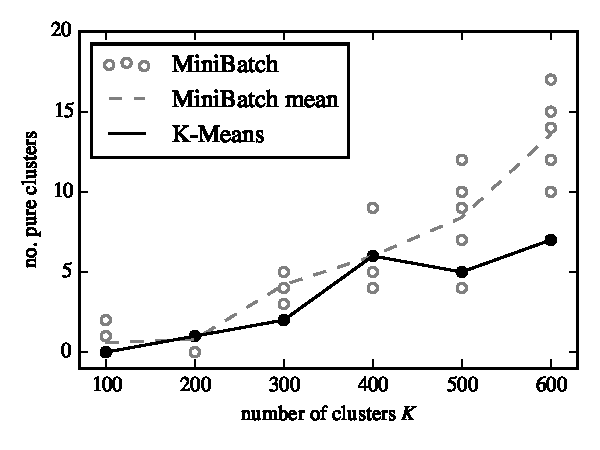
\includegraphics[width=\textwidth]{k-vs-mb-svd-len.pdf}
  \caption{Number of pure clusters vs $K$ in $K$-Means and MiniBatch $K$-Means}
  \label{fig:k-vs-mb-svd-len}
\end{subfigure}
\caption{The performance of $K$-Means and MiniBatch $K$-Means on the reduced document space with $k=150$}
\label{fig:kmeans-vs-minibatch-svd}
\end{figure}


We can observe that as $K$ increases, the number of interesting clusters increases
(see fig.~\ref{fig:k-vs-mb-svd-len}).
Therefore, we try a wide range of larger $K$ for different $k \in \{150, 250, 350, 500\}$.
The performance in terms of discovered pure clusters does not depend much on the 
rank $k$ of the reduced space (see fig.~\ref{fig:k-vs-kmeans-len-nodef}). In fact, 
it is very hard to distinguish different lines because they are quite perplexed. 
The maximum for is achieved at $K \approx 10000$ for all $k$.

\begin{figure}[h!]
\centering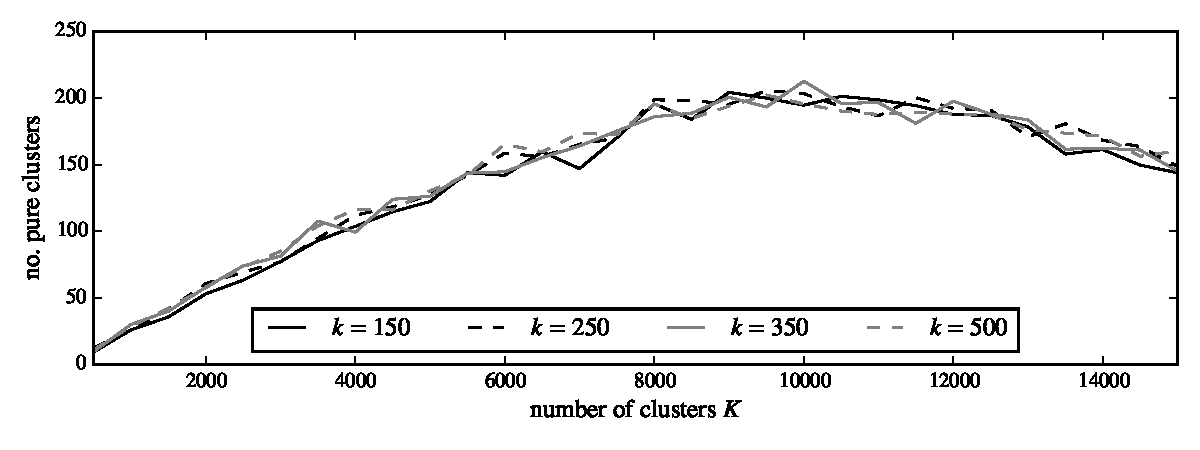
\includegraphics[width=0.9\textwidth]{k-vs-kmeans-len-nodef.pdf}
\caption{Number of discovered pure clusters in $K$-Means for different number of clusters $K$ and rank $k$.}
\label{fig:k-vs-kmeans-len-nodef}
\end{figure}

\begin{table}[h!]
\centering
\begin{tabular}{|c|c|c|}
  \hline
  Name & Size & Purity \\
  \hline
Astronomical catalogues & 53 & 0.9811 \\
Quantum mechanics & 14 & 0.9286 \\
Electrochemistry & 12 & 0.8333 \\
Particle physics  & 10 & 0.8000 \\
Partial differential equations  & 10 & 0.8000 \\
Electromagnetism  & 10 & 1.0000 \\
Topology  & 10 & 0.9000 \\
Measure theory  & 8 & 0.8750 \\
Propositional calculus  & 8 & 0.8750 \\
Baseball statistics  & 7 & 0.8571 \\
Group theory  & 7 & 0.8571 \\
Abstract algebra & 6 & 0.8333 \\
\hline
\end{tabular}
\caption{Top namespace-defining clusters discovered by $K$-Means with $K=9500$ on LSA-space with $k=250$}
\label{tab:nodef-kmeans-lsa}
\end{table}

A clustering obtained with $K=9500$ and $k=250$ discovered 213 namespace-defining
clusters (see table~\ref{tab:nodef-kmeans-lsa}), which is significantly better 
than the baseline. Let us consider a namespace
defined by the Measure Theory cluster with 8 documents, where 7 articles in
this cluster are from ``Measure theory'' category, and all the documents share
the $\mu$ identifier (see table~\ref{tab:nodef-kmeans-lsa-measuretheory}).

\begin{table}[h!]
\centering
\begin{subtable}{0.65\textwidth}
\centering
\begin{tabular}{|c|c|}
\hline
Article Name & Identifiers \\
\hline
Signed measure & $\Sigma, E, d, f, l, n, P, R, t, x, N, \nu, \mu$ \\
Ergodicity & $\Sigma,E,g,H,n,T,X,\mu, t$ \\
Support (measure theory) & $\Sigma,D,g,f,C,T,L,R,U,t,\lambda,\mu,d$ \\
Convergence of measures & $d,g,f,\mu_n,l,n,P,S,R,\eta,t,\nu,\mu$ \\
\begin{tabular}[x]{@{}c@{}} Riesz�Markov�Kakutani \\ representation theorem \end{tabular}
   & $E,d,f,\psi,K,\alpha,U,X,x,\mu$ \\
Invariant measure & $\Sigma, B,\phi,f,\mu,S,R,t,x,b,T$ \\
Fernique's theorem & $E,l_*,G,k,l,\alpha,t,x,\mu,d$ \\
Gauge symmetry & $E,d_\nu,J,L,U,W,\nu,\mu$ \\
\hline
\end{tabular}
\label{tab:nodef-kmeans-lsa-measuretheory-docs}
\caption{Identifiers and articles of the ``Measure Theory'' cluster (some identifiers are removed)}
\end{subtable}% mask EOL
\begin{subtable}{0.3\textwidth}
\centering
\begin{tabular}{|c|c|c|}
\hline
ID & Definition & Score\\
\hline
$C$ & closed set & 0.95 \\
$f$ & measurable function & 3.50 \\
$t$ & measurable & 1.64 \\
$\Sigma$ & sigma algebra & 1.86 \\
$\alpha$ & form & 0.87 \\
$\lambda$ & measure & 0.96 \\
$\mu$ & measure & 11.16 \\
$\mu_n$ & measure & 0.97 \\
$\nu$ & nonnegative measure & 0.96 \\
$\phi$ & monoid & 0.91 \\
$\psi$ & positive linear functional & 1.89 \\
\hline
\end{tabular}
\label{tab:nodef-kmeans-lsa-measuretheory-ids}
\caption{Definitions in ``Measure Theory'' (some definitions are removed)}
\end{subtable}
\caption{A namespace-defining cluster about Measure Theory discovered by $K$-Means 
with $K=9500$ and $k=250$}
\label{tab:nodef-kmeans-lsa-measuretheory}
\end{table}


\begin{table}[h!]
\centering
\begin{tabular}{|c|c|c|c|}
  \hline
  \multicolumn{4}{|c|}{$\mu$}\\
  \hline
  Size & Namespace Name & Definition & Score \\
  \hline
7 & Baseball statistics & dissociation constant & 0.89 \\
5 & Bletchley Park & motor wheels & 4.51 \\
3 & Continuous distributions & mean & 4.52 \\
5 & Fluid dynamics & dynamic viscosity & 0.99 \\
3 & Force & entropy & 0.93 \\
3 & Force & permeability & 3.63 \\
5 & General relativity & vierbein field & 0.95, \\
3 & General relativity & reduced mass & 1.79 \\
3 & Machine learning & hyperparameter & 0.86 \\
5 & Mathematical analysis & measure & 3.69 \\
5 & Mathematical finance & brownian motion & 0.84 \\
8 & Measure theory & measure & 11.16 \\
6 & Measure theory & assumptions & 0.93 \\
3 & Mechanics & modulus & 0.89 \\
3 & Molecular physics & absorption coefficient & 0.95 \\
5 & Orbits & semi-major axis & 0.89 \\
4 & Physics & numerator & 0.95 \\
4 & Probability distributions & ratio & 0.96 \\
4 & Probability theory & mean & 0.95 \\
6 & Quantum field theory & gamma matrices & 1.73 \\
14 & Quantum mechanics & molecular dipole operator & 0.96 \\
4 & Quantum mechanics & magnetic moment & 0.97 \\
3 & Quantum mechanics & magnetic dipole moment & 0.9 \\
5 & Quantum mechanics & chemical potential & 0.96 \\
3 & Quantum mechanics & formal limit & 0.95 \\
4 & Set theory & order type & 0.97 \\
3 & Special functions & partitions & 0.99 \\
3 & Stars & angular rate & 0.96 \\
6 & Statistical theory & true mean & 1.79 \\
3 & Statistical theory & standard deviation & 1.90 \\
4 & Stochastic processes & expectation & 0.96 \\
3 & Stochastic processes & time t & 0.99 \\
4 & Structural engineering & kinetic energy & 0.93 \\
6 & Theoretical physics & covariant derivative & 0.89 \\
4 & Theory of relativity & expression a\_$\mu$b & 0.93 \\
3 & Theory of relativity & four-velocity & 0.87 \\
3 & Thermodynamics & chemical potential & 1.88 \\
\hline
\end{tabular}
\caption{Definitions of $\mu$ in the namespaces discovered by $K$-Means with $K=9500$
and SVD with $k=250$ (some identifier/definition pairs are removed).}
\label{tab:nodef-kmeans-mu}
\end{table}


It is also interesting to look at all the occurrences of identifier $\mu$ in 
the results, and see how it is defined
across different namespace-defining cluster (see table~\ref{tab:nodef-kmeans-mu}).  
We can note several problems. First, sometimes there are namespaces with the same 
name, but $\mu$ stands for different things there, for example, for namespaces
``Force'' probably either ``entropy'' or ``permeability'' is not assigned correctly. 
Second, there are clearly incorrect definitions such as ``assumptions'' 
for the ``Measure theory'' namespace. Also, there are non-definitions such 
as ``expression a\_$\mu$b'' or ``time t'' assigned to $\mu$. And finally, 
some namespaces are questionable, e.g. ``Bletchley Park''. But overall
it does discover many definitions correctly, for example, ``measure'',
``mean'', ``expectation'' and others.


\begin{figure}[h!]
\centering
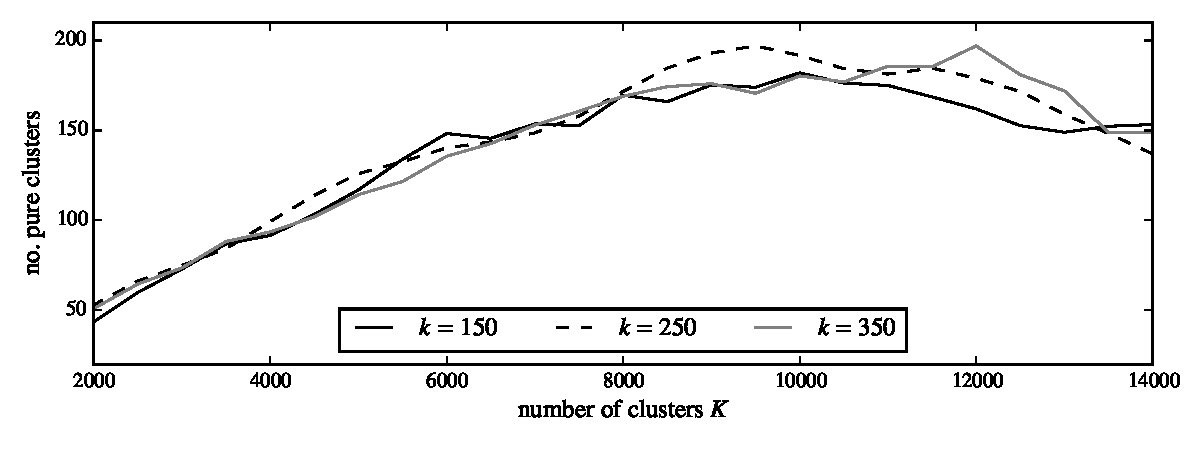
\includegraphics[width=0.9\textwidth]{k-vs-kmeans-len-nmf-nodef.pdf}
\caption{Number of discovered pure clusters in $K$-Means and NMF for different number of clusters $K$ and rank $k$.}
\label{fig:k-vs-kmeans-len-nmf-nodef}
\end{figure}

\begin{table}[h!]
\centering
\begin{tabular}{|c|c|c|}
  \hline
  Name & Size & Purity \\
  \hline
Astronomical catalogues  & 53 & 0.9811 \\
Complex analysis  & 18 & 0.8333 \\
Quantum mechanics  & 12 & 0.8333 \\
Mathematical analysis  & 10 & 0.8000 \\
Physics  & 9 & 0.8889 \\
Thermodynamics  & 6 & 0.8333 \\
Astronomical catalogues of stars  & 6 & 1.0000 \\
Knot theory  & 6 & 1.0000 \\
Stochastic processes  & 6 & 1.0000 \\
Physics  & 6 & 0.8333 \\
Stochastic processes  & 6 & 1.0000 \\
Statistics  & 6 & 0.8333 \\
\hline
\end{tabular}
\caption{Top namespace-defining clusters discovered by $K$-Means with $K=9500$ on NMF-space with $k=250$}
\label{tab:nodef-nmf}
\end{table}

\begin{table}[h!]
\centering
\begin{subtable}{0.65\textwidth}
\centering
\begin{tabular}{|c|c|}
\hline
Article Name & Identifiers \\
\hline
Pivotal quantity & $\zeta,\theta,\nu,\mu,\rho,\sigma,N,X_2,X_1,x,z,...$ \\
Errors and residuals & $\sigma,\chi,X_n,\epsilon_i,X_i,n,X_1,X,N,\mu,S_n,...$ \\
Prediction interval & $\epsilon_i,X_i,\alpha,\gamma,\beta,\mu,s_n,\sigma,E,\Phi,...$ \\
Cochran's theorem & $\mu,\sigma,B,\chi,R,U,T,Y,X,k,j,Q_2,Q_1,...$ \\
Skewness & $\gamma,m_3,\kappa,\nu,\mu,\sigma,E,F,s,u,t,...$ \\
Variance & $\Sigma, \text{SS}_\text{within},\theta,\lambda,\mu,\rho,\sigma,E,f,...$ \\
\hline
\end{tabular}
\caption{Identifiers and articles of the ``Measure Theory'' cluster (some identifiers are removed)}
\label{tab:nodef-nmf}
\end{subtable}% mask EOL
\begin{subtable}{0.3\textwidth}
\centering
\begin{tabular}{|c|c|c|}
\hline
ID & Definition & Score\\
\hline
$E$ & non-central moment & 0.92 \\
$F$ & cumulative distribution function & 0.89 \\
$f$ & probability density function & 0.99 \\
$s$ & sample variance & 3.66 \\
$\lambda$ & exponential distribution & 1.79 \\
$\mu$ & variance & 3.52 \\ 
$\rho$ & correlation & 0.99 \\
$\sigma$ & standard deviation & 4.61 \\
\hline
\end{tabular}
\caption{Definitions in ``Measure Theory'' (some definitions are removed)}
\label{tab:nodef-nmf-def}
\end{subtable}
\caption{A namespace-defining cluster about Measure Theory discovered by $K$-Means
with $K=9500$ and $k=250$}
\label{tab:nodef-nmf-stat}
\end{table}

\begin{table}[h!]
\centering
\begin{tabular}{|c|c|c|c|}
  \hline
  \multicolumn{4}{|c|}{$\mu$}\\
  \hline
  Size & Namespace Name & Definition & Score \\
  \hline
4 & Abstract algebra & lebesgue measure & 0.83 \\
4 & Algebraic curves & first & 0.93 \\
3 & Condensed matter physics & magnetic permeability & 0.99 \\
3 & Coordinate systems & form & 1.81 \\
3 & Differential equations & invariant measure & 2.73 \\
3 & Doppler effects & spatial resolution & 0.95 \\
6 & Dynamical systems & tent map & 1.71 \\
5 & Dynamical systems & entropy & 0.93 \\
6 & Electromagnetism & permeability & 1.90 \\
4 & Electromagnetism & gauge condition & 0.99 \\
4 & Financial markets & drift rate & 0.89 \\
3 & Force & th-component & 0.95 \\
3 & Functions and mappings & lebesgue measure & 0.91 \\
3 & Gravitation & semi-major axis & 0.89 \\
3 & Group theory & tate module & 1.76 \\
3 & Magnetism & magnetic moment & 1.90 \\
5 & Measure theory & measure & 8.15 \\
6 & Multivariable calculus & measure & 1.82 \\
5 & Numerical analysis & step size & 0.93 \\
6 & Physical chemistry & chemical potential & 2.57 \\
3 & Probability distributions & confidence interval & 2.77 \\
3 & Probability distributions & laplace & 3.42 \\
3 & Probability distributions & scale factor & 1.84 \\
4 & Probability theory & mean & 0.95 \\
5 & Quantum field theory & field & 0.81 \\
12 & Quantum mechanics & gamma matrices & 1.78 \\
6 & Quantum mechanics & magnetic moment & 0.87 \\
3 & Quantum mechanics & mass & 0.89 \\
3 & Solid state engineering & charge & 0.93 \\
6 & Statistical theory & known mean & 0.99 \\
6 & Statistics & variance & 3.52 \\
3 & Statistics & mean & 1.85 \\
6 & Stochastic processes & time t & 0.99 \\
6 & Stochastic processes & free rate & 0.95 \\
3 & Stochastic processes & expectation & 0.96 \\
5 & Systems theory & earths gravity & 0.93 \\
3 & Telecommunications engineering & yield & 0.93 \\
4 & Theories of gravitation & indices & 1.94 \\
3 & Theory of relativity & velocity component & 0.93 \\
\hline
\end{tabular}
\caption{Definitions of $\mu$ in the namespaces discovered by $K$-Means with $K=9500$
and NMF with $k=250$ (some identifier/definition pairs are removed).}
\label{tab:nodef-nmf-mu}
\end{table}


When \textbf{Non-Negative Matrix Factorization} is used for LSA, the results are
similar to the results, obtained by SVD (see fig.~\ref{fig:k-vs-kmeans-len-nmf-nodef}),
however for NMF the results obtained by different $k$-rank approximations
are not as perplexed as for SVD and $k=250$ does better on $K=[8000; 12000]$
than $k=150$ and $k=350$. For example, $K$-Means with $K=9500$ and $k=250$
discovered a clustering with 200 namespace-defining clusters.
The found clusters are slightly different. For example, there is no ``Measure Theory''
cluster of size 8 as in the results, found by SVD (see table~\ref{tab:nodef-kmeans-lsa}).
Let us instead consider a namespace defined by the cluster ``Statistics''
(see table~\ref{tab:nodef-nmf-stat}): there are 6 documents in the cluster
(see table~\ref{tab:nodef-nmf})
and about 43 identifier-definition in the namespace defined by the cluster
(see table~\ref{tab:nodef-nmf-def}). Note that in this cluster $\mu$ is not
assigned correctly: it is defined as ``variance'' instead of ``mean''.
If we look at all definitions of $\mu$ in this clustering (see 
table~\ref{tab:nodef-nmf-mu}) we see that, although the problems are the 
same as with decomposition by SVD, the found definitions are different. However
the difference is likely to be because of non-convexity of $K$-Means 
rather than some crucial difference in the way the matrix are factorized.




We see that generally clustering works better on reduced spaces.




In the experiments above we used $\log \text{TF} \times \text{IDF}$. Let us compare
the effect of different weighting on the resulting clusters. We will use SVD 
with $k=150$ and smaller $K$ because it is computationally faster to compute. 
We can observe that performance of $K$-Means does not depend significantly on
the weighting system when no definitions are used (see fig.~\ref{fig:nodef-weighing}).


\begin{figure}[h!]
\centering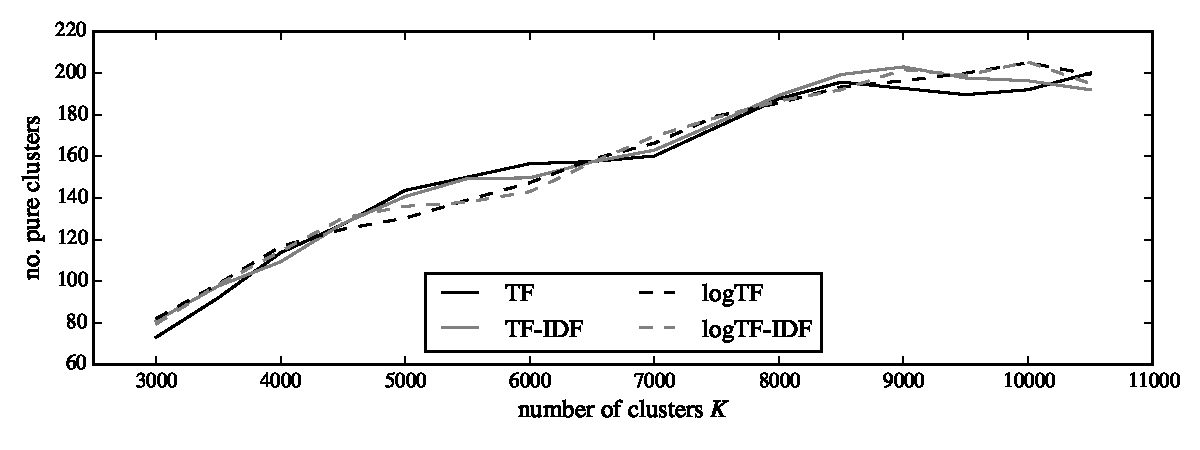
\includegraphics[width=0.9\textwidth]{nodef-weighing.pdf}
\caption{The effect of using different weighting systems on $K$-Means with SVD.}
\label{fig:nodef-weighing}
\end{figure}



\subsubsection{Weak Association} \ \\

The identifier-document matrix has the dimensionality $10419 \times 22512$, 
and there are 485\,337 elements in the matrix, so the density is about 0.002.

We do not attempt to use hierarchical methods and start with DBSCAN. 

\underline{DBSCAN SNN}

$k = 10$
dist = jaccard

$\varepsilon$=7 points
MinPts=5 points

In general doesn't give clusters


TODO add some numbers and graphs

\underline{DBSCAN}
k=15, eps=8, min\_pts=5

\begin{table}[h!]
\centering
\begin{tabular}{|c|c|}
\hline
Article & Identifiers \\
\hline
Codex Ephraemi Rescriptus  & $P, \text{papyrus}$ \\
Categories of New Testament manuscripts    & $P, \text{papyrus}$ \\
Papyrus 4  & $P, \text{papyrus}$ \\
Uncial 0308    & $P, M, \text{papyrus}, \text{47}$ \\
Codex Athous Lavrensis & $P, \text{papyrus}$ \\
Papyrus 92 & $P, \text{papyrus}$ \\
Papyrus 90 & $P, \text{papyrus}$ \\
Papyrus 111    & $P, \text{papyrus}$ \\
Uncial 0243    & $P, \text{papyrus}$ \\
Minuscule 1739 & $P, \text{papyrus}$ \\
Minuscule 88   & $P, \text{papyrus}$ \\
Authorship of the Epistle to the Hebrews   & $P, \text{papyrus}$ \\
Egerton Gospel & $P, \text{papyrus}$ \\
Rylands Library Papyrus P52    & $P, \text{papyrus}$ \\
Codex Vaticanus    & $P, \text{papyrus}$ \\
... & ... \\
\hline
\end{tabular}
\caption{Papyrus cluster by DBSCAN}
\label{tab:ssn-papyrus}
\end{table}


With  \textbf{MiniBatch $K$-Means} applied on the plain untransformed document 
space we are able to find some interesting clusters, but it general, similarity to the no-definition case, the does not show good results overall. Therefore we 
apply it to the LSA space reduced by \textbf{SVD}, when identifier-document matrix 
is reduced to rank $k$. We search for
the best combination trying $K = [500; 15000]$ and $k \in \{150, 250, 350\}$. 
Unlike the case where no definitions are used, the space produced by the 
soft definition association is affected by $k$ (see fig.~\ref{fig:k-vs-kmeans-len-svd-soft})
and the results produced by $k = 350$ are almost always better.
The weighing scheme used for this experiment is $(\log \text{TF}) \times \text{IDF}$.


\begin{figure}[h!]
\centering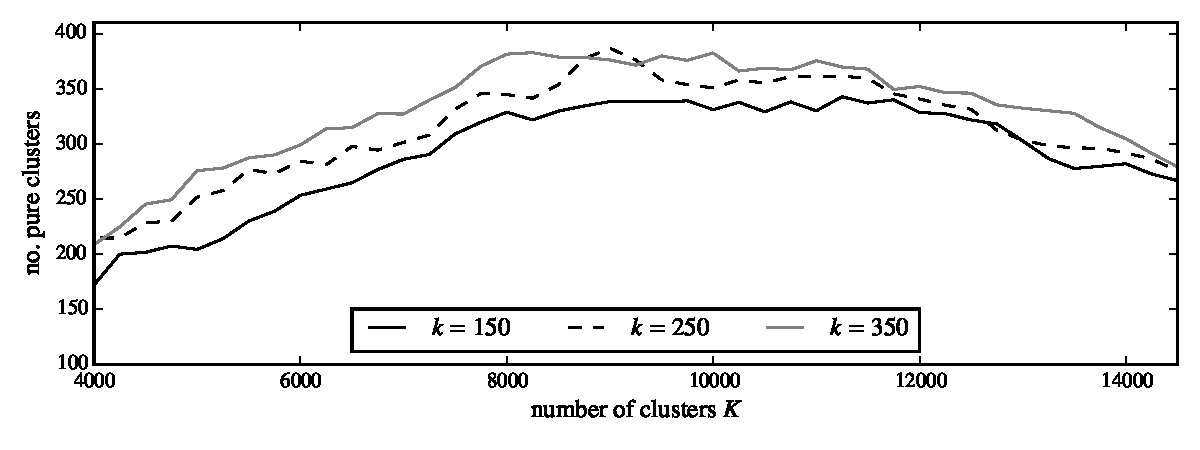
\includegraphics[width=0.9\textwidth]{k-vs-kmeans-len-svd-soft.pdf}
\caption{Number of discovered pure clusters in $K$-Means and SVD for different number of clusters $K$ and rank $k$.}
\label{fig:k-vs-kmeans-len-svd-soft}
\end{figure}

\begin{table}[h!]
\centering
\begin{tabular}{|c|c|c|}
  \hline
  Name & Size & Purity \\
  \hline
Astronomical catalogues & 53 & 0.9811 \\
Statistics & 20 & 0.8500 \\
Category theory & 16 & 0.8125 \\
Electromagnetism & 12 & 0.8333 \\
Thermodynamics & 11 & 0.8182 \\
Mathematical analysis & 11 & 0.8182 \\
Graph theory & 10 & 0.9000 \\
Graph algorithms & 10 & 0.8000 \\
Fluid dynamics & 10 & 1.0000 \\
Numerical analysis & 9 & 0.8889 \\
Group theory & 9 & 1.0000 \\
Stochastic processes & 9 & 1.0000 \\
Measure theory & 8 & 1.0000 \\
\hline
\end{tabular}
\caption{Top namespace-defining clusters discovered by $K$-Means with $K=9750$ on LSA-space with $k=350$}
\label{tab:soft-kmeans-svd}
\end{table}

\begin{table}[h!]
\centering
\begin{subtable}{0.7\textwidth}
\centering
\begin{tabular}{|c|c|}
  \hline
  Article & Identifiers \\
  \hline
Diagonalizable matrix & $v_1,\lambda_1,v_k,\lambda_3,\lambda_2,\lambda_i,\lambda_k,\lambda_j,\lambda_n,...$\\
Eigenvalues and eigenvectors & $v_i,\mu_A,\lambda_i,d,\lambda_n,...$ \\
Principal axis theorem & $v_1,u_1,\lambda_1,\lambda_2,D,S,u,...$ \\
Eigendecomposition of a matrix & $\lambda,\lambda_1,\lambda,\lambda_2,\lambda_k,R,U,T,...$ \\
Min-max theorem & $\sigma,u_n,u_k,u_i,u_1,\alpha,\lambda_1,\lambda,\lambda_i,...$ \\
Linear independence & $\Lambda,v_j,u_2,v_3,u_n,\lambda_1,\lambda_3,\lambda_2,...$ \\
Symmetric matrix & $\Lambda,\lambda_1,\lambda_2,D,Q,P,\lambda_i,...$ \\
\hline
\end{tabular}
\caption{Wiki Articles in the cluster ``Linear Algebra''}
\label{tab:soft-kmeans-la}
\end{subtable}% mask EOL
\begin{subtable}{0.3\textwidth}
\centering
\begin{tabular}{|c|c|c|}
\hline
ID & Definition & Score\\
\hline
$D$ & diagonal matrix & 1.81 \\
$t$ & real argument & 0.99 \\
$u$ & eigenvalues & 0.89  \\
$u_i$ & eigenvector & 0.89  \\
$v_1$ & eigenvectors & 1.86  \\
$\Lambda$ & diagonal matrix & 2.65  \\
$\lambda$ & eigenvalue & 0.85 \\
$\lambda_1$ & eigenvalues & 3.66 \\
$\lambda_2$ & eigenvalues & 1.76 \\
$\lambda_3$ & eigenvalues & 0.83 \\
$\lambda_i$ & eigenvalue & 4.40 \\
\hline
\end{tabular}
\caption{Definitions in ``Linear Algebra''}
\label{tab:soft-kmeans-la-def}
\end{subtable}
\caption{A ``Linear Algebra'' cluster found by $K$-Means with $K=9000$ and $k=250$.}
\label{tab:soft-kmeans-lsa}
\end{table}

\begin{table}
\centering
\begin{tabular}{|c|c|c|c|}
  \hline
  \multicolumn{4}{|c|}{$\sigma$}\\
  \hline
  Size & Namespace Name & Definition & Score \\
  \hline
3 & Algebra & multiplicity & 0.93 \\
4 & Analysis of variance & marquardt & 1.71 \\
3 & Applied and interdisciplinary physics & wavelength & 4.52 \\
6 & Cartographic projections & longitude & 10.02 \\
3 & Cartography & longitude & 7.24 \\
3 & Category theory & natural isomorphisms & 0.84 \\
4 & Condensed matter physics & penetration depth & 0.95 \\
5 & Continuous distributions & affine parameter & 0.99 \\
3 & Coordinate systems & longitude & 2.74 \\
3 & Differential equations & differential operator & 0.89 \\
8 & Differential geometry & vector fields & 1.82 \\
7 & Electronic amplifiers & typical value & 0.93 \\
3 & Electrostatics & unit length & 0.93 \\
10 & Fluid dynamics & wavelength & 6.44 \\
6 & Fluid dynamics & free path & 0.93 \\
3 & Infinity & limit ordinals & 2.68 \\
7 & Linear algebra & eigenvalue & 0.85 \\
5 & Linear algebra & matrix & 0.87 \\
3 & Linear algebra & eigenvalue & 2.53 \\
3 & Liquids & relaxation time & 0.88 \\
3 & Materials science & rate & 0.95 \\
3 & Mathematical analysis & eigenvalue & 0.86 \\
3 & Mathematical theorems & poisson distribution & 0.87 \\
4 & Measure theory & lebesgue measure & 0.95 \\
3 & Measurement & order & 0.89 \\
8 & Mechanics & previous expression & 0.95 \\
4 & Mechanics & power series & 0.88 \\
3 & Metalogic & empty word & 0.96 \\
7 & Number theory & partition & 1.90 \\
4 & Number theory & modular lambda function & 0.99 \\
3 & Operator theory & algebraic multiplicity & 0.95 \\
5 & Optics & wavelength & 1.76 \\
5 & Partial differential equations & constants & 0.87 \\
4 & Physical optics & wavelength & 3.59 \\
5 & Physics & exciton state & 2.76 \\
6 & Probability distributions & references & 0.89 \\
4 & Quantum field theory & coupling constant & 1.94 \\
5 & Quantum mechanics & wavelength & 6.47 \\
5 & Quantum mechanics & state & 2.66 \\
3 & Radioactivity & decay & 1.82 \\
4 & Representation theory of Lie groups & weight & 7.11 \\
3 & Riemannian geometry & contravariant vector field & 0.96 \\
4 & Rubber properties & engineering strain & 8.96 \\
3 & Statistical data types & regularization parameter & 0.96 \\
20 & Statistics & words & 0.93 \\
3 & Statistics & expectation & 0.99 \\
3 & Stellar astronomy & mean free path & 0.92 \\
3 & Surface chemistry & ideal gas & 0.83 \\
3 & Theoretical physics & eigenvalue & 2.71 \\
5 & Theories of gravitation & dicke & 0.95 \\
3 & Wave mechanics & wavelength & 2.65 \\
\hline
\end{tabular}
\caption{Some of definitions of $\sigma$ in the clustering obtained with $K$-Means.}
\label{tab:soft-kmeans-lambda}
\end{table}

The best result in this scheme is 414 namespace-defining clusters
(ten times better than the baseline), and it is achieved by $K$-Means
with $K=9750$ and $k=350$. The purity of this clustering is $0.63$.
Let us consider a ``Linear Algebra'' cluster (table~\ref{tab:soft-kmeans-lsa})
with 6 documents and some of extracted definitions in documents
of this cluster, and all these articles share identifers $\lambda_1$, $m$ and $n$.
Let us consider all definitions of identifier ``$\lambda$''. In total, there 
are 93 clusters where $\lambda$ is used (see table~\ref{tab:soft-kmeans-lambda}), 
and in many cases it is possible to determine that the assignment is correct 
(e.g. ``eigenvalue'', ``wavelength'', ``regularization parameter''). 
Some cases are not correct, for example, when we have clusters with the same name
where $\lambda$ denotes different things (e.g. in two ``Quantum Mechanics'' clusters),
or in the case of ``Linear Algebra'' cluster where it denotes a matrix. 


\subsubsection{Strong Association}

$37879 \times 22512$ sparse identifier-document matrix with 499070 entries, 
so the density of this matrix is just 0.00058.



Best result found with Mini-Batch $K$-Means is 350 - slightly worse than 
in the Soft Association. 

Add graphs



\subsubsection{Russian Wikipedia} \ \\

Apply the best method for Russian Wiki




\subsection{Building Hierarchy} \label{sec:hierarchy}


After the namespaces are found, we need to organize them into a hierarchical
structure. It is hard to do automatically, and we choose to use
existing hierarchies for mathematical knowledge, and then map the
found namespaces to these hierarchies.

The first hierarchy that we use is ``Mathematics Subject Classification'' (MSC)
hierarchy \cite{ams2010msc} by the American Mathematical Society, and it
is used for categorizing mathematical articles. In this scheme there are
64 top-level categories such as ``Mathematical logic'', ``Number theory'',
or ``Fourier analysis''. It also includes some physics categories such
as ``Fluid mechanics'' or ``Quantum Theory''. The following top level
categories are excluded: ``General'', ``History and biography'' and
``Mathematics education''.

Each top-level category contains second-level categories and third-level
categories. In this work we exclude all subcategories those code
ends with 99: they are usually ``Miscellaneous topics'' or
``None of the above, but in this section''.

Additionally, we excluded the following second level categories because
they interfere with PACS, a hierarchy for Physics:

\begin{itemize}
\item Quantum theory $\to$ Axiomatics, foundations, philosophy
\item Quantum theory $\to$ Applications to specific physical systems
\item Quantum theory $\to$ Groups and algebras in quantum theory
\item Partial differential equations $\to$ Equations of mathematical physics and other areas of application
\end{itemize}


% \begin{itemize}
% \item Statistics $\to$ Sufficiency and information
% \item Functional analysis $\to$ Other (nonclassical) types of functional analysis
% \item Functional analysis $\to$ Miscellaneous applications of functional analysis
%\end{itemize}

The second hierarchy is ``Physics and Astronomy Classification Scheme'' (PACS)
\cite{aps2010pacs}, which is a scheme for categorizing articles about Physics.
Like in MSC, we remove the top-level category  ``GENERAL''.

Finally, we also use the ACM Classification Scheme \cite{rous2012acm}
available as a SKOS \cite{miles2005skos} ontology at their website \cite{amc2012ccs}.
The SKOS ontology graph was processed with RDFLib \cite{rdflib}.
We use the following top level categories:
``Hardware'', ``Computer systems organization'', ``Networks'',
``Software and its engineering'', ``Theory of computation'',
``Information systems'', ``Security and privacy'',
``Human-centered computing'', ``Computing methodologies''.

After obtaining and processing the data, the three hierarchies
are merged into one.


However these categories are only good for English articles and
a different hierarchy is needed for Russian. One of such hierarchies is
``����\-���\-�����\-��� ���\-��\-��\-��� ������-���\-��\-���\-��� �����\-��\-���''
(�����)~-- ``State categorizator of scientific and technical information'', which
is a state-recommended scheme for categorizing scientific articles published
in Russian  \cite{feodosimov2000grnti}. The hierarchy  is extracted from the
official website\footnote{\url{http://grnti.ru/}}. It provides
a very general categorization and therefore we keep only the following math-related
categories: ``����������'' (``Astronomy''), ``��������'' (``Biology''),
``�����������'' (``Informatics''), ``����������'' (``Mathematics''),
``��������'' (``Mechanics''), ``���\-���\-����'' (``Statistics''),
``������'' (``Physics''), ``�����'' (``Chemistry''),
``���������. ������������� �����'' (``Economics'') and others.


One we a hierarchy is established, each found namespace is mapped to
the most suitable second-level category. This is done by keywords matching.
First, we extract all key words from the category, which includes
top level category name, subcategory name and all third level categories.
Then we also extract the category information from the namespace, but
we also use the names of the articles that form the namespace.
Finally, the keyword matching is done by using the cosine similarity
between the cluster and each category. The namespace is assigned to the
category with the best (largest) cosine score.

If the cosine score is low (below $0.2$) or there is only one
keyword matched, then the cluster is assigned to the ``OTHERS''
category.

For example, consider a namespace  derived from the cluster consisting of
``Tautology (logic)'', ``List of logic systems'', ``Regular modal logic''
``Combinational logic'' documents. Among others, these articles belong to categories
``Mathematical logic'' and ``Logic''. Then the following is the list of keywords
extracted from the cluster:
``tautology'', ``logic'', ``list'', ``systems'', ``regular'', ``modal'', ``combinational'',
``logical'', ``expressions'', ``formal'', ``propositional'', ``calculus'' and so on.
Apparently, this namespace is about mathematical logic.

Then consider a list of keywords for ``'General logic'', a subcategory of
``Mathematical logic and foundations'' from MSC:
``mathematical'', ``logic'', ``foundations'', ``general'', ``classical'', ``propositional'', ``type'', ``subsystems'' and others.

These keywords are represented as vectors in some Vector Space and the cosine score
between these vectors is calculated. For this example, the cosine is
approximately 0.75, and this is the largest similarity, and therefore this namepsace
is mapped to the ``General logic'' subcategory.

Unfortunately the mapping is not always correct (TODO: add examples)


\subsection{Java Language Processing} \label{sec:jlp}

Previously we have illustrated the idea of identifier namespaces by comparing
it with namespaces in Computer Science, and it allowed us to develop an intuition
behind the namespaces in mathematics and also propose a method to discover them:
we motivated the assumption that there exist ``namespace defining'' 
groups of documents by arguing that these groups also exist in 
programming languages.
In this section we will try to do the reserve: apply the methods 
developed for identifier namespace discovery to the source code. 

If a programming language is statically typed, like Java or Pascal,
usually it is possible to know the type of a variable from the declaration
of this variable. Therefore we can see variable names as ``identifiers''
and variable types as ``definitions''. Clearly, there is a difference
between variable types and identifier definitions, but we believe
that this comparison is valid because the type carries additional semantic
information about the variable and in what context it can be used --
like the definition of an identifier.

The information about variables and their types can be extracted from a
source code repository, and each source file can be processed to
obtain its Abstract Syntax Tree (AST). By processing the ASTs,
we can extract the variable declaration information. Thus, each
source file can be seen as a document, which is represented
by all its variable declarations.

In this work we process Java source code, and for parsing it
and building ASTs we use a library JavaParser \cite{javaparser}.
The Java programming language was chosen because it requires the programmer
to always specify the type information when declaring a variable.
It is different for other languages when the type information is
usually inferred by the compilers at compilation time.


In Java a variable can be declared in three places:
as an inner class variable (or a ``field''), as a method (constructor)
parameter or as a local variable inside a method or a constructor.
We need to process all three types of variable declarations
and then apply additional preprocessing, such as converting the name
of the type from short to fully qualified using the information from the
import statements. For example, \verb|String| is converted to
\verb|java.lang.String| and \verb|List<Integer>| to \verb|java.util.List<Integer>|,
but primitive types like \verb|byte| or \verb|int| are left unchanged.


Consider an example in the listing~\ref{code:javaclass}. There is a
class variable \texttt{threshold}, a method parameter \texttt{in} and
two local variables \texttt{word} and \texttt{posTag}. The following
relations will be extracted from this class: (``threshold'', \verb|double|),
(``in'', \verb|domain.Word|), (``word'', \verb|java.lang.String|),
(``posTag'', \verb|java.lang.String|).
Since all primitives and classes from packages that start with
\verb|java| are discarded, at the end the class \verb|WordProcesser|
is represented with only one relation (``in'', \verb|domain.Word|).


\begin{lstlisting}[language=Java,caption={A Java class},label={code:javaclass}]
package process;

import domain.Word;

public class WordProcesser  {

    private double threshold;

    public boolean isGood(Word in) {
        String word = in.getWord();
        String posTag = in.getPosTag();
        return isWordGood(word) && isPosTagGood(posTag);
    }

    // ...

}
\end{lstlisting}


In the experiments we applied this source code analysis to
the source code of Apache Mahout 0.10 \cite{mahout}, which is an open-source
library for scalable Machine Learning and Data Mining.
As on \today, this dataset consists of 1\,560 java classes with 45\,878
variable declarations. After discarding declarations from the standard Java API,
primitives and types with generic parameters, only 15\,869 declarations were
retained.

The following is top-15 variable/type declarations extracted from the Mahout 
source code:

\begin{itemize}
\item ``conf'', \verb|org.apache.hadoop.conf.Configuration| (491 times)
\item ``v'', \verb|org.apache.mahout.math.Vector| (224 times)
\item ``dataModel'', \verb|org.apache.mahout.cf.taste.model.DataModel| (207 times)
\item ``fs'', \verb|org.apache.hadoop.fs.FileSystem| (207 times)
\item ``log'', \verb|org.slf4j.Logger| (171 times)
\item ``output'', \verb|org.apache.hadoop.fs.Path| (152 times)
\item ``vector'', \verb|org.apache.mahout.math.Vector| (145 times)
\item ``x'', \verb|org.apache.mahout.math.Vector| (120 times)
\item ``path'', \verb|org.apache.hadoop.fs.Path| (113 times)
\item ``measure'', \verb|org.apache.mahout.common.distance.DistanceMeasure| (102 times)
\item ``input'', \verb|org.apache.hadoop.fs.Path| (101 times)
\item ``y'', \verb|org.apache.mahout.math.Vector| (87 times)
\item ``comp'', \verb|org.apache.mahout.math.function.IntComparator| (74 times)
\item ``job'', \verb|org.apache.hadoop.mapreduce.Job| (71 times)
\item ``m'', \verb|org.apache.mahout.math.Matrix| (70 times)
\end{itemize}

We used the ``soft'' association method to incorporate ``definition'' 
(i.e. types), and considering each source code file as a document, 
we build an identifier-document matrix of dimensionality 
$1436 \times 1560$. Only identifiers that occur at least twice are used 
to build the matrix. 

Previously the best performance was achieved by using LSA and MiniBatch $K$-Means, 
and therefore we apply the same algorithms here. However there are a lot of instances 
of the types \texttt{Vector} and \texttt{Matrix}, and to mediate its influence, we use two variants of TF-IDF:
with usual TF component and with sublinear TF. 
The best performance is achieved with the rank $k=200$ of SVD and 
number of clusters $K=200$ using sublinear weighting (see fig.~\ref{fig:jlp-perf}).
% each experiment was repeated 10 times and we record the average


\begin{figure}[h!]
\centering
\hfill
\begin{subfigure}[b]{0.47\textwidth}
  \centering
  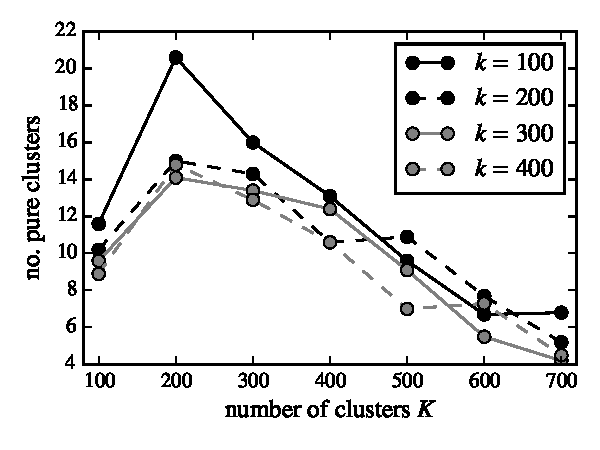
\includegraphics[width=\textwidth]{jlp-lens.pdf}
  \caption{Usual TF $\times$ IDF weighting}
  \label{fig:jlp-perf-tf}
\end{subfigure}
~
\begin{subfigure}[b]{0.47\textwidth}
  \centering
  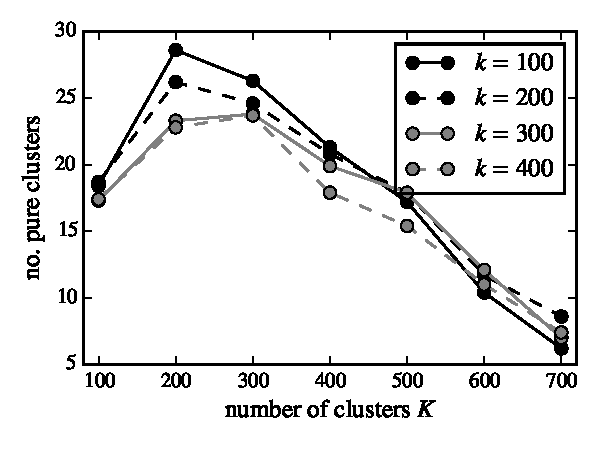
\includegraphics[width=\textwidth]{jlp-lens-sublin.pdf}
  \caption{Sublinear TF $\times$ IDF weighting}
  \label{fig:jlp-perf-subtf}
\end{subfigure}
\caption{The performance MiniBatch $K$-Means on the Mahout dataset.}
\label{fig:jlp-perf}
\end{figure}


With these parameters the best result is 33 clusters. 
One of such clusters is a cluster about SVD: there are 5 classes 
from the \verb|recommender.svd|\footnote{full name: \texttt{org.apache.mahout.cf.taste.impl.recommender.svd}} package
(\texttt{Factorization}, \texttt{FilePersistenceStrategy}, \texttt{NoPersistenceStrategy}, \texttt{PersistenceStrategy}, \texttt{FilePersistenceStrategyTest})
and one from \verb|kddcup.track1.svd|\footnote{full name: \texttt{org.apache.mahout.cf.taste.example.kddcup.track1.svd}} package
(\texttt{Track1SVDRunner})
Although this cluster is not 100\% pure, in the sense that not all of 
these classes belong to the same package, these classes are 
clearly related: they are all about SVD.
The top dimensions with the most influence in this cluster are 
\verb|svd.Factorization|\footnote{full name: \texttt{org.apache.mahout.cf.taste.impl.recommender.svd.Factorization}} 
and \texttt{factorization}.

% One of these 
% clusters is \verb|org.apache.mahout.math.neighborhood| cluster with  
% BruteSearch, FastProjectionSearch, LocalitySensitiveHashSearch, ProjectionSearch, 
% Searcher, LocalitySensitiveHashSearchTest, SearchSanityTest. All these classes are
%related. Not all classes from this package are included. For example, 
% HashedVector and LumpyData are not, and, judging by the name of these
%classes, they appear a bit different from the rest. Therefore 
%these classes are indeed semantically related. 
% There are many identifiers in this namespace


Note that there is a difference between mathematical namespaces and
namespaces discovered in the source code. The found ``namespaces'' do not necessarily
correspond to the real packages in the source code. The reason for this is 
the document-centric view on the namespaces: for documents we assume that the 
namespaces are not directly observed, and instead we can see only the documents where 
these namespaces are used. It is not the case for real namespaces 
in software: we do observe namespaces directly, and documents (that is, classes) 
are also the elements of the namespaces. 



\subsection{Result Analysis and Experiment Conclusions}


Hierarcical methods are too slow, and SLINK is not good.
Bisecting $K$-Means is good for explaining steps but not very practical

MiniBatch K means is preferred to usual KMeans:
fast but same results

The baseline of random cluster assignment is beaten.

NMF takes a lot of time to decompose a matrix with large
$k$

 $k=100$ 30 min, but with results inferior to SVD
 $k=250$ 2 hours, with results comparable to SVD

The complexity of NMF is $O(kn)$


The best definition embedding technique is soft association.
The best clsutering algorithm is $K$-Means with $K=9500$
on the semantic space produced by rank-reduced SVD with $k = 250$
with TF-IDF weight where TF is sublinear.







\section{Evaluation}



\section{Conclusions}

The goal of this work was to discover namespaces in mathematical notation
given a collection of documents with mathematical formulae. To achieve that,
we used document clustering techniques on documents, where each document is 
represented by identifiers, used in its formulae. 

We expected to discover namespaces, that are homogenies and corresponded
to the same area of knowledge. The clusters that we discovered are homogenous, 
but not all corresponded to the same category. This is why we 
additionally used the category information to recognize the namespaces-defining
clusters amount all clusters, and then we built namespaces from them.

We also initially expected that there would be more namespace-defining clusters, 
but in our results the majority of clusters are not ``pure'': documents inside these 
clusters do not belong to the same category. These clusters are only homogenous in 
the cluster analysis sense: the within-cluster distances is minimal. 


Nevertheless, the obtained results indicate that there are namespaces in mathematical 
notation and it is possible to discover them automatically from a collection of 
documents. We also verified that clustering document is better than random guessing 
by the factor of ten. We observed that dimensionality reduction techniques 
are very helpful, and clustering algorithms work better on the reduce space. 
MiniBatch $K$-Means algorithms shows the best results for discovering 
namespace-defining clusters.

There are many ways in which the present approach can be improved further.
In the next section we discuss possible directions.


\section{Outlook and Future Work}

\subsection{Implementation and Other Algorithms}  % \ \\

We use the Probabilistic approach to extracting definitions for identifiers, and
it is good because it requires almost no parameter tuning.
While this approach works well most of the time, sometimes we observe
some false positives, most likely due to the fact that the dataset is
quite noisy. It potentially can be improved by using some Machine Learning
method, which, however, may require creating a hand-labeled dataset
with identifier-definition relations. To facilitate the creation of such a
dataset it is possible to pre-generate some data using using the current approach
for further labeling.

In the experiments section we have observed that cluster algorithms that produce
many clusters tend to have good performance. However, they also tend to create related
clusters from the same category and with same or similar identifiers and
definitions. Therefore such results can be refined further and merged.
This can be done, for example, by using the join operation from
the Scatter/Gather algorithm \cite{cutting1992scatter}, which finds the most
similar clusters and merges them.

We were not able to apply hierarchical agglomerative clustering algorithms because
their time complexity is prohibitive, but they may produce good clusters.
For these algorithms we are usually interested in the nearest neighbors of a given
data point, and therefore we can use approximation algorithms for computing nearest
neighbors such as Locality-Sensitive Hashing (LSH) \cite{leskovec2014mining}.
The LSH algorithms can be used for text clustering \cite{ravichandran2005randomized},
and therefore they should work well for identifiers. Additionally, LSH is also a
dimensionality reduction technique, and we have observed that generally
reducing dimensionality helps to obtain better clusters.

In this work we use hard assignment clustering algorithms, which means, that a document
can import only from one namespace. This assumption does not necessarily always hold true
and we may model the fact that documents may import from several namespaces by
using Fuzzy Clustering (or Soft Clustering) algorithms \cite{baraldi1999survey}.

In Latent Semantic Analysis other dimensionality reduction techniques
can be used, for example, Local Non-Negative Matrix Factorization \cite{li2001learning}.
There is also a randomized Non-Negative Matrix Factorization algorithm that uses
random projections \cite{wang2010efficient} \cite{damle2014random},
which potentially can give a speed up while not significantly losing
in performance. Another dimensionality reduction technique useful for
discovering semantics is Dynamic Auto-Encoders \cite{mirowski2010dynamic}.

Additionally, we can try different approaches to clustering such as
Spectral Clustering \cite{ng2002spectral} or Micro-Clustering \cite{uno2015micro}.

Finally, topic modeling techniques such as Latent Dirichlet Allocation
\cite{blei2003latent} can be quite useful for modeling namespaces. It can be
seen as a ``soft clustering'' technique and it can naturally model the fact that
a document may import from several namespaces.


\subsection{Other Concepts} %  \ \\
% Other concepts

In this work we assume that document can import only from one namespace,
but in reality is should be able to import from several namespaces. As discussed,
it can be modeled by Fuzzy Clustering. But it also can be achieved by
dividing the document in parts (for example, by paragraphs)
and then treating each part as an independent document.

For document clustering we only use identifiers, extracted definitions
and categories. It is possible to take advantage of additional information from
Wikipedia articles. For example, extract some keywords from the articles
and use them to get a better cluster assignment.

The Wikipedia data set can be seen as a graph, where two articles have
an edge if there is an interwiki link between them. Pages that describe
certain namespaces may be quite interconnected, and using this idea it is possible
to apply link-based clustering methods (such as ones described in
\cite{botafogo1991identifying} and \cite{johnson1996adaptive}) to find namespace
candidates. There are also hybrid approaches that can use both textual representation
and links \cite{oikonomakou2005review}.

Vector Space Model is not the only possible model to represent textual
information as vectors. There are other ways to embed textual information
into vector spaces like word2vec \cite{mikolov2013efficient} or
GloVe \cite{pennington2014glove}, and these methods may be useful
for representing identifers and definitions as well.

Tensors may be a better way of representing
identifier-definition pairs. For example, we can represent the data set
as a 3-dimensional tensor indexed by documents, identifiers and definition.
Tensor Factorization methods for revealing semantic information
are an active area of research in NLP and linguistics \cite{anisimov2014semantic},
so it is also possible to apply these methods to the namespace discovery problem.

Finally, while running experiments, we observed that sometimes results of
clustering algorithms with the same parameters produce quite different
results, or some algorithms produce a small amount of good quality namespaces,
while others produce many namespaces which may be less coherent.
Therefore it can be interesting to investigate how to combine the results
of different cluster assignments such that the combined result is better
in terms of the number of namespace-defining clusters. One way of
achieving this can be building ensembles of clustering algorithms \cite{strehl2003cluster}.
Alternatively, a special approach for optimizing for the number of pure clusters
can be proposed, for example, partially based on the ideas from
Boosting \cite{freund1996experiments}: apply a clustering algorithm,
remove the discovered pure clusters, and run the algorithm again on the remaining
documents until no new clusters are discovered.


\subsection{Other Datasets} % \ \\
% Other Datasets

In this work we use Wikipedia as the data source and extract namespaces from the
English part of Wikipedia. Additionally, we also apply the methods to the Russian
part, and therefore it shows that it is possible to extract namespaces from
Wikipedia in any other available language.

But we can also apply to some other larger dataset, such as arXiv\footnote{\url{http://arxiv.org/}}, a repository of over one million
of scientific papers in many different areas. The source code of these
articles are available in \LaTeX, and it can be processed automatically.

There are many scientific Q\&A websites on the Internet. The stack
exchange\footnote{\url{http://stackexchange.com/}} is one of the largest Q\&A networks,
and there are many sites on this network that contain mathematical formulae, such as
``mathematics'', ``mathoverflow'', ``cross validated'', ``data science'',
``theoretical computer science'', ``physics'', ``astronomy'', ``economics'' and many others.
This network makes their data available for download and it also can be a good
data source for namespace discovery. In addition to content, the questions contain
a lot of potentially useful metadata such as related questions and tags.


\subsection{Unsolved Questions} % \ \\

The most important question is how to extend this method to situations when
no additional information about document category is known. To solve
it, we need to replace the notion of purity with some other objective
for discovering namespace-defining clusters.

Also, a metric for evaluating the quality of a namespace is needed.
Now we assume that pure clusters are namespace-defining clusters. But the namespace
candidates should adhere to the namespace definition as much as possible,
and therefore a good criteria is needed to quantify to what extent the definition
is satisfied. This will help to define whether a cluster defines a good namespace
or not.

After namespaces are discovered we organize them into hierarchies.
To do that we use existing hierarchies, but they are not always complete
and there are mismatches. What is more, when this technique is applied to some
other language, a different hierarchy is needed for this language, and we experienced
it when processing the Russian part of Wikipedia: for that we needed to obtain
a special hierarchy. There should be a way of building these hierarchies
automatically, without the need of external dataset.
Potentially it should be possible to use hierarchical clustering
algorithms, but it may result in very deep and unnatural hierarchies, and
therefore some additional investigation in this direction may be needed.



\section{Bibliography}

\bibliographystyle{plain}
\bibliography{bibliography}


\end{document} 